% === Revtex Declaration ===
\documentclass[aps, 10pt, english, twoside, pra, nofootinbib, longbibliography]{revtex4-1}

% === All of the Packages I use frequently ===
\usepackage{../packages/shared}

% === Drafting Declarations ===
\draftprofile[TC Fraser]{TC}{Red}
\draftprofile[Elie Wolfe]{E}{Green}

% === Numbering For amsthm theorem environments ===
\theoremstyle{plain}
\newtheorem{theorem}{Theorem}
\newtheorem{lemma}[theorem]{Lemma}

\theoremstyle{definition}
\newtheorem{definition}[theorem]{Definition}
\newtheorem{example}[theorem]{Example}

\theoremstyle{remark}
\newtheorem{remark}[theorem]{Remark}

% === Commonly re-occurring symbols ===
\newcommand{\hgraph}{\mathcal{H}}
\newcommand{\graph}{\mathcal{G}}
\newcommand{\nodes}{\mathcal{N}}
\newcommand{\weights}{\mathcal{W}}
\newcommand{\edges}{\mathcal{E}}
\newcommand{\trans}{\mathcal{T}}
\newcommand{\ind}{\mathcal{I}}
\newcommand{\perm}{\Omega}
\newcommand{\Hilb}{\mathcal{H}}
\newcommand{\ancestralindep}{\perp}
\newcommand{\valprod}{\circ}
% When I introduce a new term or definition
\newcommand{\term}[1]{\textcolor{Mahogany}{\textbf{#1}}}

% === Mathematical operators that are denoted with words ===
\newcommand{\setoperator}[1]{%
\expandafter\DeclareDocumentCommand\csname#1\endcsname{O{} O{} m}{{\mathsf{#1}_{##1}^{##2}\!}\br{##3}}%
}

\setoperator{Pa} % Parents of a node
\setoperator{Ch} % Children of a node
\setoperator{An} % Ancestry of a node
\setoperator{Sub} % subgraph
\setoperator{AnSub} % Ancestral subgraph
\setoperator{Ext} % Extension of outcomes
\setoperator{Com} % Compatible equivalence relation
\setoperator{Nec} % Necessary nodes
\setoperator{UnNec} % Unnecessary nodes
\setoperator{Inj} % injectable sets
\setoperator{ImInj} % images of the injectable sets
\setoperator{PreInj} % Pre-injectable sets
\setoperator{Aut} % graph automorphism
\setoperator{Orb} % Group Orbits
\setoperator{Perm} % Permutation group

\newcommand{\outc}[1]{o\!\bs{#1}} % Fritz's BBTII notation for observed outcomes
\DeclareDocumentCommand{\prob}{O{} O{}}{\ifthenelse{\equal{#1}{}}{P}{P_{#1}}\ifthenelse{\equal{#2}{}}{}{\!\br{#2}}} % probability distribution
\DeclareDocumentCommand{\probvec}{O{} O{}}{\ifthenelse{\equal{#1}{}}{\mathcal{P}}{\mathcal{P}_{#1}}\ifthenelse{\equal{#2}{}}{}{\!\br{#2}}} % probability distribution vector

% === To allow for labeling of rows and columns of a matrix ===
\usepackage{../packages/kbordermatrix}
\renewcommand{\kbldelim}{(} % Left delimiter
\renewcommand{\kbrdelim}{)} % Right delimiter

% === Causal structure formatting for tikz ===
% =========================
% Causal Structure Diagrams
% =========================
\definecolor{obs_outline}{RGB}{51,157,215}
\definecolor{obs_fill}{RGB}{222,253,255}
\definecolor{obs_text}{RGB}{0,0,0}
\definecolor{lat_outline}{RGB}{251,141,54}
\definecolor{cause}{RGB}{30, 0, 30}
\definecolor{lat_fill}{RGB}{255,213,153}
\definecolor{lat_text}{RGB}{0,0,0}
\tikzset{square/.style={regular polygon,regular polygon sides=4}}
\tikzset{triangle/.style={regular polygon,regular polygon sides=3}}
\tikzset{observed/.style={obs_text, align=center, triangle, thick, draw=obs_outline, fill=obs_fill, inner sep=-0.2em, text width=1.5em}}
\tikzset{latent/.style={lat_text, align=center, circle, thick, draw=lat_outline, fill=lat_fill, text width=1.5em, inner sep=0.2em}}
\tikzset{fade/.style={opacity=0.2}}
\tikzset{unfade/.style={opacity=1.0}}
% TikZ stile to apply keys only on specific beamer overlays
% onslide=<overlay spec>{key=value, key=value, ...}
\tikzset{onslide/.code args={<#1>#2}{%
  \only<#1>{\pgfkeysalso{#2}}%
}}
\providecommand{\p}[1]{#1}
% \tikzset{cause/.style={mid arrow/.style={postaction={decorate,decoration={markings, mark=at position .5 with {\arrow[#1]{stealth}}}}},}}
\tikzset{
    % style to apply some styles to each segment of a path
    on each segment/.style={
        decorate,
        decoration={
            show path construction,
            moveto code={},
            lineto code={
                \path [#1]
                (\tikzinputsegmentfirst) -- (\tikzinputsegmentlast);
            },
            curveto code={
                \path [#1] (\tikzinputsegmentfirst)
                .. controls
                (\tikzinputsegmentsupporta) and (\tikzinputsegmentsupportb)
                ..
                (\tikzinputsegmentlast);
            },
            closepath code={
                \path [#1]
                (\tikzinputsegmentfirst) -- (\tikzinputsegmentlast);
            },
        },
    },
    % style to add an arrow in the middle of a path
    mid arrow/.style={postaction={decorate,decoration={
                markings,
                mark=at position .6 with {\arrow[scale=1.5, cause]{stealth}}
            }}},
}
% =========================
% =========================

\begin{document}
    \title{Inequalities Witnessing Quantum Incompatibility in The Triangle Scenario}
    \author{Thomas C. Fraser}
    \email{tcfraser@tcfraser.com}
    \affiliation{Perimeter Institute for Theoretical Physics, Waterloo, Ontario, Canada \\ University of Waterloo, Waterloo, Ontario, Canada}
    % \author{Elie Wolfe}
    % \email{ewolfe@perimeter@institute.ca}
    % \affiliation{Perimeter Institute for Theoretical Physics, Waterloo, Ontario, Canada}
    \date{\today}
    \begin{abstract}
        Causal inference aims to identify which observable distributions are compatible with a given causal structure. Compatibility inequalities for the triangle scenario have been obtained and demonstrated to be violated by quantum configurations. Obtaining these inequalities has lead to the development of new computational techniques suitable for large causal structures with numerous outcomes. Numerical optimizations against these inequalities have found new quantum configurations that are incompatible with the triangle scenario, potentially suggesting new quantum resources qualitatively different from those known previously. \todo[TC]{Write a better abstract.}
    \end{abstract}
    \maketitle
    \tableofcontents

    \section{Introduction}
    \todo[TC]{Discuss why the marginal problem is important.}
    \section{Definitions \& Notation}
    \comment[TC]{This entire section should be integrated into the body when logical to do so.}
    \begin{definition}
        Borrowing the notation from \cite{Fritz_2014}, each random variable $v$ has a set of all possible outcomes called the \term{outcome space} or \term{valuation space} and is denoted $O_v$. When referencing a \textit{specific} element of $O_v$ or \textit{valuation} of $v$, the notation $\outc{v}$ is used. This notation generalizes to set of random variables $V = \bc{v_1, \ldots, v_{\abs{V}}}$;
        a specific outcome of $\outc{V} \in O_V$ is used to reference a particular tuple or vector of outcomes,
        \[ \outc{V} \defined \br{\outc{v_1}, \outc{v_2}, \ldots, \outc{v_{\abs{V}}} } = \br{\outc{v}}_{v \in V} \eq \label{eq:outcomespace}\]
        It is important to note that the ordering of events in \cref{eq:outcomespace} is irrelevant. Similarly, the outcome space $O_V$ for a set of random variables $V$ is the \term{valuation product} `$\valprod$' of the individual outcome spaces,
        \[ O_V \defined O_{v_1} \valprod \cdots \valprod O_{v_{\abs{V}}} \]
        Where `$\valprod$' is defined such that for $A \cap B = \emptyset$,
        \[ \outc{A} \valprod \outc{B} \defined \br{\outc{a_1}, \ldots, \outc{a_{\abs{A}}}, \outc{b_1}, \ldots, \outc{b_{\abs{B}}}} = \br{\outc{v}}_{v \in A \cup B} \]
        Often `$\valprod$' will be omitted where there is little ambiguity. When referencing the probability that a set of variables $V$ has outcome $\outc{V}$ (say $v_1 = 0, v_2 = 3$), we intend for the following class of notations to be used interchangeably.
        \[ \prob[V][\outc{V}] = \prob[][\outc{V}] = \prob[][\outc{v_1}\outc{v_2}] = \prob[][v_1 = 0, v_2 = 3] = \prob[][v_2 = 3, v_1 = 0] = \prob[v_1, v_2][03] \]
    \end{definition}

    \begin{definition}
        \label{def:extendable}
        An outcome $\outc{V}$ is said to be \term{extendable} to an outcome $\outc{W}$ (where $V \subseteq W$) if there exists an outcome $\outc{W\setminus V}$ such that $\outc{W} = \outc{W\setminus V} \valprod \outc{V}$.
        \[ \Ext{\outc{V} \to \outc{W}} \iff \exists \outc{W\setminus V} \mid \outc{W} = \outc{W\setminus V} \valprod \outc{V} \]
        The idea being that a \textit{less specific} outcome $\outc{V}$ can be made \textit{more specific} by assigning outcomes to the remaining random variables in $W \setminus V$. If such an outcome $\outc{W\setminus V}$ exists, it is unique.
    \end{definition}

    \begin{definition}
        The set of all extendable outcomes of $\outc{V}$ in $O_{W}$ is called the \term{extendable set} and can be written as,
        \[ \Ext[W]{\outc{V}} \defined \outc{V} \valprod O_{W\setminus V} \defined \bc{\outc{W} \in O_{W} \mid \Ext{\outc{V} \to \outc{W}}} \]
        The extendable set of $\outc{V}$ in $W$ is the set of all outcomes of $O_W$ that \textit{agree} with $\outc{V}$ about valuations for variables in $V$. In this language, two outcomes $\outc{V}$ and $\outc{W}$ are \term{compatible} if they are both extendable to some outcome $\outc{V \cup W}$. Equivalently, $\outc{V}$ and $\outc{W}$ agree on their valuations of $V \cap W$.
        \[ \Com{\outc{V}, \outc{W}} \iff \exists \outc{V \cup W} \mid \Ext{\outc{V} \to \outc{V \cup W}}, \Ext{\outc{W} \to \outc{V \cup W}} \]
    \end{definition}

    \begin{example}
        Consider two sets of random variables $V = \bc{a, b}$ and $W = \bc{a, b, c}$. Clearly $V \subseteq W$; a prerequisite for extendability. Also take all individual outcome spaces to be finite and of order 3: $O_a = O_b = O_c = \bc{1,2,3}$. Then $\outc{V} = \outc{\bc{a,b}} = \br{a = 1, b = 2}$ is extendable to the outcome $\outc{W} = \br{a = 1, b = 2, c = 1}$, and the extendable set of $\outc{V}$ in $O_{W}$ is,
        \[ \Ext[a,b,c]{a = 1, b = 2} = \bc{\br{a = 1, b = 2, c = 1}, \br{a = 1, b = 2, c = 2}, \br{a = 1, b = 2, c = 3}} \]
    \end{example}

    % \begin{definition}
    %     Two outcomes $\outc{V_1}$ and $\outc{V_2}$ over two distinct sets of random variables $V_1$ and $V_2$ are called \term{accordant} or \textit{compatible} if they are mutually realizable. In terms of extendable sets, $\outc{V_1}$ and $\outc{V_2}$ are accordant if there exists an outcome $\outc{V_1 \cup V_2} \in O_{V_1 \cup V_2}$ such that,
    %     \[ \outc{V_1}, \outc{V_2} \subseteq \outc{V_1 \cup V_2}  \]
    %     Accordance between two outcomes is the \textit{opposite} of exclusive.
    % \end{definition}

    \begin{definition}
        \label{def:graph}
        A \term{graph} is an ordered tuple $\br{\nodes, \edges}$ of \textit{nodes} and \textit{edges} respectively where the nodes can represent any object and the edges are pairs of nodes. For convenience of notation, one defines an index set over the nodes denoted $\ind_\nodes$.
        \[ \nodes = \bc{n_i \mid i \in \ind_\nodes} \quad \edges = \bc{\bc{n_j, n_k} \mid j,k \in \ind_\nodes} \]
    \end{definition}

    \begin{definition}
        \label{def:directed_graph}
        A \term{directed graph} $\graph$ is an ordered tuple $\br{\nodes, \edges}$ of \textit{nodes} and \textit{edges} respectively where the nodes can represent any object and the edges are \textit{ordered} pairs of nodes. For convenience of notation, one defines an index set over the nodes denoted $\ind_\nodes$.
        \[ \nodes = \bc{n_i \mid i \in \ind_\nodes} \quad \edges = \bc{n_j \to n_k \mid j,k \in \ind_\nodes} \]
    \end{definition}

    \begin{definition}
        \label{def:graph_terms}
        The following definitions are common language in directed graph theory. Let $n, m \in \nodes$ be example nodes of the graph $\graph$.
        \begin{itemize}
            \item The \term{parents of a node}: $\Pa[\graph]{n} \defined \bc{m \mid m \to n}$
            \item The \term{children of a node}: $\Ch[\graph]{n} \defined \bc{m \mid n \to m}$
            \item The \term{ancestry of a node}: $\An[\graph]{n} \defined \bigcup_{i\in\mathbb{W}} \Pa[\graph][i]{n}$ where $\Pa[\graph][i]{n} \defined \Pa[\graph]{\Pa[\graph][i-1]{n}}$ and $\Pa[\graph][0]{n} = n$
        \end{itemize}
        All of these terms can be generalized to sets of nodes $N \subseteq \nodes$ through union over the elements,
        \begin{itemize}
            \item The \term{parents of a node set}: $\Pa[\graph]{N} \defined \bigcup_{n\in N}\Pa[\graph]{n}$
            \item The \term{children of a node set}: $\Ch[\graph]{N} \defined \bigcup_{n\in N}\Ch[\graph]{n}$
            \item The \term{ancestry of a node set}: $\An[\graph]{N} \defined \bigcup_{n\in N}\An[\graph]{n}$
        \end{itemize}
        Moreover, an \term{induced subgraph} of $\graph$ due to a set of nodes $N \subseteq \nodes$ is the graph composed of $N$ and all edges $e \in \edges$ of the original graph that are contained in $N$.
        \[ \Sub[\graph]{N} \defined \br{N, \bc{e_i \mid i \in \ind_\edges, e_i \subseteq N}}\]
        An \term{ancestral subgraph} of $\graph$ due to $N \subseteq \nodes$ is the induced subgraph due to the ancestry of $N$.
        \[ \AnSub[\graph]{N} \defined \Sub[\graph]{\An[\graph]{N}} \]
    \end{definition}

    \begin{definition}
        \label{def:dag}
        A \term{directed acyclic graph} or \term{DAG} $\graph$ is an directed graph \cref{def:directed_graph} with the additional property that no node $n$ is in its set of \term{ancestors}.
        \[ \forall n \in \nodes : n \notin \bigcup_{i\in\mathbb{N}} \Pa[\graph][i]{n}\]
        Notice the difference between using the natural numbers $\mathbb{N}$ to distinguish \textit{ancestors} from \textit{ancestry}.
    \end{definition}

    \begin{definition}
        \label{def:hypergraph}
        A \term{hypergraph} denoted $\hgraph$ is an ordered tuple $\br{\nodes, \edges}$ of \textit{nodes} and \textit{hyperedges} respectively where the nodes can represent any object and the hyperedges are \textit{subsets} of nodes. For convenience of notation, one defines an index set over the nodes and hyperedges of a hypergraph $\hgraph$ denoted $\ind_\nodes$ and $\ind_\edges$ respectively.
        \[ \hgraph = \br{\nodes, \edges} \quad \nodes = \bc{n_i \mid i \in \ind_\nodes} \quad \edges = \bc{e_i \mid i \in \ind_\edges, e_i \subseteq \nodes} \]
        Note that whenever the hyperedge or node index is arbitrary, it will be omitted. There is a dual correspondence between hyperedges $e \in \edges$ and nodes $n \in \nodes$ in a Hypergraph. A hyperedge $e$ is viewed as a set of nodes $\bc{n_i}$, and a node $n$ can be viewed as the set of hyperedges $\bc{e_i}$ that contain it.
    \end{definition}

    \begin{definition}
        \label{def:hgraph_trans}
        A \term{hypergraph transversal} (or edge hitting set) $\trans$ of a hypergraph $\hgraph$ is a set of nodes $\trans \subseteq \nodes$ that have non-empty intersections with every hyperedge in $\edges$.
        \[ \trans = \bc{n_i \in \nodes \mid i \in \ind_\trans } \quad \forall e \in \edges : \trans \cap e \neq \emptyset \]
    \end{definition}

    \begin{definition}
        A \term{necessary node} of a transversal $\trans$ is a node $n$ such that $\trans \setminus n$ is no longer a valid transversal. The set of all necessary nodes is denoted $\Nec{\trans}$,
        \[ \Nec{\trans} = \bc{n \in \trans \mid \exists e \in \edges : \br{\trans \setminus n} \cap e = \emptyset} \]
        An \term{unnecessary node} of a transversal $\trans$ is any node that is \textit{not} necessary. The set of all unnecessary nodes is denoted $\UnNec{\trans}$,
        \[ \UnNec{\trans} = \trans \setminus \Nec{\trans} \]
        A \term{minimal hypergraph transversal} $\trans$ is any valid transversal of $\hgraph$ where every node $n$ is \textit{necessary}.
        \[ \trans = \Nec{\trans} \]
    \end{definition}

    \begin{definition}
        A \term{weighted hypergraph} $\hgraph_\weights$ is a regular hypergraph satisfying \cref{def:hypergraph} equipped with a set of weights $\weights$ ascribed to each node such that a weighted hypergraph is written as a triplet $\br{\weights, \nodes, \edges}$.
        \[ \weights = \bc{w_i \mid i \in \ind_\nodes, w_i \in \R} \]
        One would say that a particular node $n_i$ carries weight $w_i$ for each $i \in \ind_\nodes$.
    \end{definition}

    \begin{definition}
        A \term{bounded transversal} of a weighted hypergraph $\hgraph_\weights$ is a transversal $\trans$ of the unweighted hypergraph $\hgraph$ and a real number $t$ (denoted $\trans_{\leq t}$) such that the sum of the node weights of the transversal is bounded by $t$.
        \[ \trans_{\leq t} = \bc{n_i \mid i \in \ind_\trans} \quad \text{s.t.} \sum_{j\in\ind_\trans} w_j \leq t \]
        One can definte analogous \term{(strictly) upper/lower bounded transversals} by considering modifications of the notation: $\trans_{< t}, \trans_{\geq t}, \trans_{> t}$.
    \end{definition}

    \begin{definition}
        A \term{causal structure} is simply a DAG with the extra classification of each node into one of two categories; the \term{latent nodes} and \term{observed nodes} denoted $\nodes_L$ and $\nodes_O$. The latent nodes correspond to random variables that are either hidden through some fundamental process or cannot/will not be measured. The observed nodes are random variables that are measurable. Every node is either latent or observed and no node is both:
        \[ \nodes_L \cap \nodes_O = \emptyset \qquad \nodes_L \cup \nodes_O = \nodes \]
    \end{definition}

    \begin{definition}
        The \term{product distribution} two distributions is denoted as usual with $\times$ and is defined as,
        \[ \br{\prob[v] \times \prob[w]}\br{\outc{v}, \outc{w}} \defined \prob[v][\outc{v}]\prob[w][\outc{w}] \]
        A product distribution of $k$ distributions is defined recursively,
        \[ \prod_{i=1}^{k} \prob[v_i] \defined \br{\prob[v_1] \times \cdots \times \prob[v_k]} \]
    \end{definition}

    \begin{definition}
        The \term{marginalization} of a distribution $\prob[v \cup w]$ to the distribution $\prob[v]$ is denoted $\sum_{w} \prob[v \cup w] = \prob[v]$ and is defined such that,
        \[ \forall \outc{v} \in O_v : \br{\sum_{w} \prob[v, w]}\br{\outc{v}} \defined \sum_{o\bs{w} \in O_w} \prob[v, w][\outc{v}, \outc{w}] \]
    \end{definition}

    \begin{definition}
        Following common notation used in \cite{Fritz_2011}, we use the notation $\bs{k} = \br{1, \ldots, k}$ to be a finite index set. Moreover, when referencing a finite set with $k$ elements, we can write,
        \[ A_{\bs{k}} \defined \bc{A_i}_{i \in \bs{k}} = \bc{A_1, \ldots, A_k} \]
    \end{definition}

    \todo[TC]{How many definitions do I need to write??}

    \section{Triangle Scenario}
    \todo[TC]{Discuss the Triangle Scenario, previous work done on it, etc.}

    Figure 8 of Appendix E \cite{Henson_2014}
    Figure 1 of \cite{Inflation}


    Focusing on the inflation depicted in \cref{fig:inflated_triangle_scenario}, we obtained the maximally pre-injectable sets through the procedure outlined in \cite{Inflation}.
    \begin{equation*}
        \eq \label{eq:pre-injectable_triangle_scenario}
        \begin{gathered}
            \textbf{Maximal Pre-injectable Sets} \\
            \bc{A_1, B_1, C_1, A_4, B_4, C_4} \\
            \bc{A_1, B_2, C_3, A_4, B_3, C_2} \\
            \bc{A_2, B_3, C_1, A_3, B_2, C_4} \\
            \bc{A_2, B_4, C_3, A_3, B_1, C_2} \\
            \bc{A_1, B_3, C_4} \\
            \bc{A_1, B_4, C_2} \\
            \bc{A_2, B_1, C_4} \\
            \bc{A_2, B_2, C_2} \\
            \bc{A_3, B_3, C_3} \\
            \bc{A_3, B_4, C_1} \\
            \bc{A_4, B_1, C_3} \\
            \bc{A_4, B_2, C_1}
        \end{gathered}
        \qquad
        \begin{gathered}
            \textbf{Ancestral Independences} \\
            \bc{A_1, B_1, C_1} \ancestralindep \bc{A_4, B_4, C_4} \\
            \bc{A_1, B_2, C_3} \ancestralindep \bc{A_4, B_3, C_2} \\
            \bc{A_2, B_3, C_1} \ancestralindep \bc{A_3, B_2, C_4} \\
            \bc{A_2, B_4, C_3} \ancestralindep \bc{A_3, B_1, C_2} \\
            \bc{A_1} \ancestralindep \bc{B_3} \ancestralindep \bc{C_4} \\
            \bc{A_1} \ancestralindep \bc{B_4} \ancestralindep \bc{C_2} \\
            \bc{A_2} \ancestralindep \bc{B_1} \ancestralindep \bc{C_4} \\
            \bc{A_2} \ancestralindep \bc{B_2} \ancestralindep \bc{C_2} \\
            \bc{A_3} \ancestralindep \bc{B_3} \ancestralindep \bc{C_3} \\
            \bc{A_3} \ancestralindep \bc{B_4} \ancestralindep \bc{C_1} \\
            \bc{A_4} \ancestralindep \bc{B_1} \ancestralindep \bc{C_3} \\
            \bc{A_4} \ancestralindep \bc{B_2} \ancestralindep \bc{C_1}
        \end{gathered}
    \end{equation*}
    As can be counted, there are $12$ maximally pre-injectable sets which will be indexed $1$ through $12$ in the order seen above ($\bc{V_1, \ldots, V_{12}}$)

    \begin{figure}
    \begin{center}
        \begin{minipage}[b]{.48\textwidth}
            \centering
            \scalebox{1.0}{\begin{tikzpicture}[scale=1]
    \begin{scope}[every node/.style=observed]
        \node (C) at (-2, 0) {$C$};
        \node (B) at (2, 0) {$B$};
        \node (A) at (0, {2*sqrt(3)}) {$A$};
    \end{scope}
    \begin{scope}[every node/.style=latent]
        \node (X) at (-1, {sqrt(3)}) {$X$};
        \node (Y) at (1, {sqrt(3)}) {$Y$};
        \node (Z) at (0, 0) {$Z$};
    \end{scope}
    \begin{scope}[every path/.style={draw=cause, thick}]
        \path[postaction={on each segment={mid arrow}}]
        (X) -- (A)
        (X) -- (C)
        (Y) -- (A)
        (Y) -- (B)
        (Z) -- (B)
        (Z) -- (C);
    \end{scope}
\end{tikzpicture}}
            \caption{The casual structure of the Triangle Scenario. Three variables $A,B,C$ are observable and illustrated as triangles, while $X, Y, Z$ are latent variables illustrated as circles.}
            \label{fig:triangle_scenario}
        \end{minipage}\hspace{0.04\textwidth}%
        \begin{minipage}[b]{.48\textwidth}
            \centering
            \scalebox{0.8}{\newcommand{\ift}{2.3}
\begin{tikzpicture}[scale=2]
    \begin{scope}[every node/.style=observed]
        \node (C4) at (-2, 0) {$C_4$};
        \node (C3) at ({-2 + 1/\ift}, {1/(\ift*sqrt(3))}) {$C_3$};
        \node (C2) at ({-2 + 2*1/\ift}, {2*1/(\ift*sqrt(3))}) {$C_2$};
        \node (C1) at ({-2 + 3*1/\ift}, {3*1/(\ift*sqrt(3))}) {$C_1$};
        \node (B4) at (2, 0) {$B_4$};
        \node (B3) at ({2 - 1/\ift}, {1/(\ift*sqrt(3))}) {$B_3$};
        \node (B2) at ({2 - 2*1/\ift}, {2*1/(\ift*sqrt(3))}) {$B_2$};
        \node (B1) at ({2 - 3*1/\ift}, {3*1/(\ift*sqrt(3))}) {$B_1$};
        \node (A4) at (0, {2*sqrt(3)}) {$A_4$};
        \node (A3) at (0, {2*sqrt(3) - 2/sqrt(3)*(1/\ift)}) {$A_3$};
        \node (A2) at (0, {2*sqrt(3) - 2*2/sqrt(3)*(1/\ift)}) {$A_2$};
        \node (A1) at (0, {2*sqrt(3) - 3*2/sqrt(3)*(1/\ift)}) {$A_1$};
    \end{scope}
    \begin{scope}[every node/.style=latent]
        \node (X2) at (-1, {sqrt(3)}) {$X_2$};
        \node (X1) at ({-1 + 1/\ift}, {sqrt(3) - 1/(\ift*sqrt(3))}) {$X_1$};
        \node (Y2) at (1, {sqrt(3)}) {$Y_2$};
        \node (Y1) at ({1 - 1/\ift}, {sqrt(3) - 1/(\ift*sqrt(3))}) {$Y_1$};
        \node (Z1) at (0, 0.5) {$Z_1$};
        \node (Z2) at (0, 0) {$Z_2$};
    \end{scope}
    \begin{scope}[every path/.style={draw=cause, thick}]
        \path[postaction={on each segment={mid arrow}}]
        (X2) -- (A4) (X2) -- (C4) (X2) -- (C2) (X2) -- (A3)
        (Y2) -- (A4) (Y2) -- (B4) (Y2) -- (A2) (Y2) -- (B3)
        (Z2) -- (B4) (Z2) -- (C4) (Z2) -- (B2) (Z2) -- (C3)
        (X1) -- (A1) (X1) -- (C1) (X1) -- (C3) (X1) -- (A2)
        (Y1) -- (A1) (Y1) -- (B1) (Y1) -- (A3) (Y1) -- (B2)
        (Z1) -- (B1) (Z1) -- (C1) (Z1) -- (B3) (Z1) -- (C2)
        ;
    \end{scope}
\end{tikzpicture}}
            \caption{An inflated causal structure of the Triangle Scenario \cref{fig:triangle_scenario}.}
            \label{fig:inflated_triangle_scenario}
        \end{minipage}
    \end{center}
    \end{figure}

    \section{Compatibility, Contextuality and the Marginal Problem}
    \label{sec:comp_con_mp}
    In order to determine if a given marginal distribution $\prob[V]$ or set of marginal distributions $\prob[V_{\bs{k}}] \defined \bc{\prob[V_1], \ldots, \prob[V_k]}$ is compatible with a causal structure $\graph$, one should first formalize what is meant by \textit{compatible}.

    \begin{definition}
        A set of \term{causal parameters} for a particular causal structure $\graph$ is the specification of a conditional distribution for every node $n \in \nodes$ given it's parents in $\graph$.
        \[ \bc{\prob[n \mid \Pa[\graph]{n}] \mid n \in \nodes} \]
    \end{definition}
    \begin{definition}
        \label{def:compatible}
        A marginal distribution $\prob[V]$ is \term{compatible} with a causal structure $\graph$ (where it is assumed that $V \subseteq \nodes_O$) if there exists a \textit{choice} of causal parameters $\bc{\prob[n \mid \Pa[\graph]{n}] \mid n \in \nodes}$ such that $\prob[V]$ can be \textit{recovered} from the following series of operations:
        \begin{enumerate}
            \item First obtain a joint distribution over \textit{all} nodes of of the causal structure,
            \[ \prob[\nodes] = \prod_{n \in \nodes} \prob[n \mid \Pa[\graph]{n}] \]
            \item Then marginalize over the latent nodes of $\graph$,
            \[ \prob[\nodes_O] = \sum_{\nodes_L} \prob[\nodes] \]
            \item Finally marginalize over the observed nodes not in $V$ to obtain $\prob[V]$,
            \[ \prob[V] = \sum_{\nodes_O \setminus V} \prob[\nodes_O] \]
        \end{enumerate}
        A set of marginal distributions $\prob[V_{\bs{k}}]$ is compatible with $\graph$ if each of the distributions can be made compatible by the \textit{same} choice of causal parameters.
        A distribution $\prob[V]$ or set of distributions $\prob[V_{\bs{k}}]$ is said to be \term{incompatible} with a causal structure if there \textit{does not exist} a set of causal parameters with the above mentioned property.

        \todo[TC]{Source this?}
    \end{definition}
    Operations 2 and 3 of \cref{def:compatible} are related to the \textit{marginal problem}.
    \begin{definition}
        \label{def:marginal_problem}
        \term{The Marginal Problem:} Given a set of distributions $\prob[V_{\bs{k}}] \defined \bc{\prob[V_1], \ldots, \prob[V_k]}$ where $V_i \subseteq \mathcal{V}$ for some set of random variables $\mathcal{V}$ and $k \geq 2$, does there exist a joint distribution $\prob[\mathcal{V}]$ such that each given distribution $\prob[V_i]$ can be obtained from marginalizing $\prob[\mathcal{V}]$?
        \[ \forall i \in \bs{k} : \prob[V_i] = \sum_{\mathcal{V} \setminus V_i} \prob[\mathcal{V}] \]
        Typically (although not strictly necessary), $\mathcal{V}$ is taken to mean the union of all $V_i$'s.
        \[ \mathcal{V} = V_1 \cup \cdots \cup V_k = \bigcup_{i\in\bs{k}} V_i \eq \label{eq:marginals_union} \]
    \end{definition}

    \todo[TC]{Mention polytope perspective and existing methods}
    \begin{definition}
        \label{def:marginal_model}
        A reoccurring motif of these discussions will be the set of distributions $\prob[V_{\bs{k}}] \defined \bc{\prob[V_1], \ldots, \prob[V_k]}$ mentioned in \cref{def:marginal_problem}. In agreement with \cite{Fritz_2011} we will call this set of distributions a \term{marginal model} and denote it $\prob_{V_{\bs{k}}}$ provided that they are \textit{compatible}:
        \[ \forall i \neq j \text{ if } V_i \cap V_j \neq \emptyset \text{ then } \sum_{V_i \setminus V_j} \prob[V_i] = \sum_{V_j \setminus V_i} \prob[V_j]  \]
        We call the set of subsets $V_{\bs{k}} \defined \bc{V_1, \ldots, V_k}$ the marginal contexts or the \term{maximal marginal scenario} $V_{\bs{k}}$\footnote{Rigorously speaking as defined by \cite{Fritz_2011}, a marginal scenario forms an \textit{abstract simplicial complex} where $V' \in V_{\bs{k}}$ whenever $V' \subseteq V_i$ for some $i$. ``Maximal'' refers to the restriction that $\forall i,j : V_i \not \subseteq V_j$.} and an individual $V_i$ a \term{marginal context}. The union of all contexts is denoted $\mathcal{V}$ and define it exactly as in \cref{eq:marginals_union}.

        Following definition 2.3 in \cite{Fritz_2011}, a marginal model is said to be \term{contextual} if it \textit{does not} admit a solution to the marginal problem and \term{non-contextual} otherwise.

        In addition, we elect to define the \term{marginal outcomes} $O_{V_{\bs{k}}}$ to be the set of all outcomes belonging to outcomes of the marginal contexts.
        \[ O_{V_{\bs{k}}} \defined O_{V_1} \cup \cdots \cup O_{V_k} = \bigcup_{i \in \bs{k}} O_{V_i} \]
        % By an intended abuse of notation, we say that a particular outcome is an ``element'' of $O_{V_{\bs{k}}}$ if it is an element of $O_{V_i}$ for some $i \in \bs{k}$.
        % \[ \outc{V_i} \in O_{V_{\bs{k}}} \]
        Note that $O_{V_{\bs{k}}}$ is \textit{not} a valid outcome space, analogous to the fact that $P_{V_{\bs{k}}}$ is \textit{not} a probability distribution. Instead $O_{V_{\bs{k}}}$ is a collection of outcome spaces just as $P_{V_{\bs{k}}}$ is a collection of distributions.
    \end{definition}

    \begin{definition}
        A \term{causal compatibility inequality} $\mathcal{I}_{V_{\bs{k}}}$ for a marginal scenario $V_{\bs{k}}$ is a probabilistic inequality that is obeyed for every compatible marginal model $\prob_{V_{\bs{k}}}$. Whenever the marginal scenario $V_{\bs{k}}$ in question is evident by context, the subscript of $\mathcal{I}_{V_{\bs{k}}}$ will be dropped leaving just $\mathcal{I}$.
    \end{definition}
    \todo[TC]{Discuss Compatibility, connection to cooperative games/resources, bell incompatibility?}
    \todo[TC]{Connection between contextuality and Compatibility via the marginal problem for causal parameters}
    \todo[TC]{Discuss what is meant by a `complete' solution to the marginal problem}
    \todo[TC]{Maybe define the possibilistic marginal problem for later}
    \section{Summary of the Inflation Technique}
    \label{sec:summary_inflation}
    The causal inflation technique, first pioneered by Wolfe, Spekkens, and Fritz \cite{Inflation} and inspired by the \textit{do calculus} and \textit{twin networks} of Ref. \cite{Pearl_2009}, is a family of causal inference techniques that can be used to determine if a probability distribution is compatible or incompatible with a given causal structure. As a preliminary summary, the inflation technique begins by \textit{augmenting} a causal structure with additional copies of its nodes, producing an \textit{inflated} causal structure, and then exposes how causal inference tasks on the inflated causal structure can be used to make inferences on the original causal structure. Copies of the original nodes are distinguished by an additional subscript called the \term{copy-index}. For example node $A$ of \cref{fig:triangle_scenario} has copies $A_1, A_2, A_3, A_4$ in the inflation of \cref{fig:inflated_triangle_scenario}. Following the notions of Ref. \cite{Inflation}, all such copies are deemed equivalent via a \term{copy-index equivalence} relation denoted `$\sim$'. A copy-index is effectively arbitrary, so $A'$ will refer to an arbitrary inflated copy of $A$.
    \[ A \sim A_1 \sim A' \not\sim B \sim B_1 \sim B' \]
    We preemptively generalize the notion of copy-index equivalence to other mathematical objects like sets, graphs, and groups by saying that $X \sim Y$ if $X = Y$ upon removal of the copy-index. Equipped with the common graph-theoretic terminology and notation of \cref{def:graph_terms}, an inflation can be formally defined as follows:
    \begin{definition}
        An \term{inflation} of a causal structure $\graph$ is another causal structure $\graph'$ such that:
        \[ \forall n' \in \nodes': \AnSub[\graph']{n'} \sim \AnSub[\graph]{n} \eq \label{eq:inflation_defn}\]
    \end{definition}
    The motivation being that since the ancestry of each node $n'$ in $\graph'$ plays the \textit{exact same} role as the ancestry of its source copy $n$ in $\graph$, then every compatible joint distribution $\prob[\nodes]$ on $\graph$ can be used to \textit{create} compatible joint distributions on $\graph'$. To do this, first notice that every compatible joint distribution $\prob[\nodes]$ uniquely defines a set of causal parameters for $\graph$.
    \[ \forall n \in \nodes : \prob[n\mid \Pa[\graph]{n}] = \sum_{\nodes \setminus n} \prob[\nodes] \eq \label{eq:unique_causal_parameters}\]
    Now since \cref{eq:inflation_defn} enforces that $\Pa[\graph']{n'} \sim \Pa[\graph]{n}$, one can create a set of \term{inflated causal parameters} using \cref{eq:unique_causal_parameters},
    \[ \forall n' \in \nodes' : \prob[n'\mid \Pa[\graph']{n'}] \defined \prob[n\mid \Pa[\graph]{n}] \]
    Which in turn uniquely defines a compatible joint distribution $\prob[\nodes']$ on $\graph'$\footnote{Of course not all compatible joint distributions on $\nodes'$ are constructed in this way; all that is demonstrated is that all joint distributions constructed in this way are compatible.}.
    \[ \prob[\nodes'] = \prod_{n' \in \nodes'} \prob[n'\mid \Pa[\graph']{n'}] \]
    This is known as the \term{weak inflation lemma}; compatible joint distributions over $\nodes$ induce compatible joint distributions over $\nodes'$. Before generalizing to the inflation lemma, a careful observation needs to be made. For any pair of subsets of nodes $N \subseteq \nodes$ and $N' \subseteq \nodes'$ that are equivalent up to copy-index $N \sim N'$, if $\AnSub[\graph]{N} \sim \AnSub[\graph']{N'}$ then any compatible \textit{marginal} distribution $\prob[N]$ over $N$ induces a compatible marginal distribution $\prob[N']$ over $N'$. In fact since $N'$ contains no duplicate nodes up to copy index (simply because $N \sim N'$ and $N$ cannot contain duplicate nodes), $\prob[N] = \prob[N']$. We refer such sets $N'$ as the \term{injectable sets} of $\graph'$ and $N$ the \term{images of the injectable sets} of $\graph$.
    \begin{align*}
        \Inj[\graph]{\graph'} &\defined \bc{N' \subseteq \nodes' \mid \exists N \subseteq \nodes : N \sim N'} \\
        \ImInj[\graph]{\graph'} &\defined \bc{N \subseteq \nodes \mid \exists N' \subseteq \nodes' : N \sim N'}
    \end{align*}

    \begin{lemma}
        \label{lem:inflation}
        \term{The Inflation Lemma} Given a particular inflation $\graph'$ of $\graph$, if a marginal model $\bc{\prob[N] \mid N \in \ImInj[\graph]{\graph'}}$ is compatible with $\graph$ then all marginal models $\bc{\prob[N'] \mid N' \in \Inj[\graph]{\graph'}}$ are compatible with $\graph'$ provided that $\prob[N] = \prob[N']$ for all instances where $N \sim N'$.
        This is lemma 3 of \cite{Inflation}.
    \end{lemma}

    The inflation lemma is the most important result of the causal inflation technique \cite{Inflation}. The contrapositive version of \cref{lem:inflation} is a powerful tool for determining compatibility. Any compatibility constraint on marginal models $\bc{\prob[N'] \mid N' \in \Inj[\graph]{\graph'}}$ of the inflated causal structure $\graph'$ correspond to valid compatibility constraints on marginal models $\bc{\prob[N] \mid N \in \ImInj[\graph]{\graph'}}$ of the original causal structure. Corollary 5 of \cite{Inflation} proves this explicitly for incompatibility inequalities $\mathcal{I}$; which the remainder of this work focuses on.  Additionally, the inflation lemma holds when considering any subset of $\Inj[\graph]{\graph'}$ (analogously $\ImInj[\graph]{\graph'}$). Therefore, in situations where latent nodes are present in $\graph$, one only needs to consider injectable sets that are composed of \textit{observable nodes}.

    In this work, we obtain inequalities that constrain the set of injectable marginal models $\bc{\prob[N'] \mid N' \in \ImInj[\graph]{\graph'}}$ for the inflated Triangle Scenario of \cref{fig:triangle_scenario} by considering the marginal problem (see \cref{sec:comp_con_mp}) for the set of \term{maximally pre-injectable sets}\footnote{The set of all pre-injectable sets forms a topological \textit{simplicial conplex}. `Maximal' refers to the pre-injectable sets that are no proper subset of another.}. As defined by \cite{Inflation}, a pre-injectable set $V$ is a subset of $\nodes'$ that can be written as the decomposed into the union of injectable sets $V = \bigcup_i N'_i$ where $\bc{N'_i \in \Inj[\graph]{\graph'}}$ that are mutually \term{ancestrally independent},
    \[ \forall i,j : N'_i \ancestralindep N'_j \iff \An[\graph']{N'_i} \cap \An[\graph']{N'_j} = \emptyset  \]
    In doing so, any distribution over all nodes of a pre-injectable set $\prob[\cup_i N'_i]$ will factorize according to graphical $d$-separation conditions \cite{Pearl_2009},
    \[ \prob[V] = \prob[\cup_i N'_i] = \prod_{i}\prob[N'_i] \]
    This turns linear inequalities over the pre-injectable distributions into polynomial inequalities over the injectable distributions, allowing one to replace all such distributions with equivalent distributions over the original random variables of $\nodes$. $\PreInj[\graph]{\graph'}$ will denote the set of all pre-injectable sets.

    \section{The Fritz Distribution}
    The \term{Fritz distribution} $P_F$ is a quantum-accessible distribution known to be incompatible with the Triangle Scenario. Explicitly, $P_F$ is a three-party ($A,B,C$), four-outcome ($1,2,3,4$) distribution that has form as follows:
    \begin{align*}
    \eq \label{eq:fritz_dist}
    \begin{split}
    \prob[F][111] = \prob[F][221] = \prob[F][412] = \prob[F][322] = \prob[F][233] = \prob[F][143] = \prob[F][344] = \prob[F][434] &= \f{1}{32}\br{2 + \sqrt{2}} \\
    \prob[F][121] = \prob[F][211] = \prob[F][422] = \prob[F][312] = \prob[F][243] = \prob[F][133] = \prob[F][334] = \prob[F][444] &= \f{1}{32}\br{2 - \sqrt{2}}
    \end{split}
    \end{align*}
    Here the notation $\prob[F][abc] = \prob[ABC][abc] = \prob[][A=a,B=b,C=c]$ is used. The Fritz distribution $\prob[F]$ can be realized with the following quantum configuration:
    \begin{equation}
    \begin{gathered}
    \label{eq:fritz_quantum_realization}
    \rho_{AB} = \ket{\Psi^+}\bra{\Psi^+} \quad \rho_{BC} = \rho_{CA} = \ket{\Phi^+}\bra{\Phi^+} \\
    M_{A} = \bc{\ket{0\psi_0}\bra{0\psi_0}, \ket{0\psi_{\pi}}\bra{0\psi_{\pi}}, \ket{1\psi_{-\pi/2}}\bra{1\psi_{-\pi/2}}, \ket{1\psi_{\pi/2}}\bra{1\psi_{\pi/2}}} \\
    M_{B} = \bc{\ket{\psi_{\pi/4}0}\bra{\psi_{\pi/4}0}, \ket{\psi_{5\pi/4}0}\bra{\psi_{5\pi/4}0}, \ket{\psi_{3\pi/4}1}\bra{\psi_{3\pi/4}1}, \ket{\psi_{-\pi/4}1}\bra{\psi_{-\pi/4}1}} \\
    M_{C} = \bc{\ket{00}\bra{00}, \ket{01}\bra{01}, \ket{10}\bra{10}, \ket{11}\bra{11}}
    \end{gathered}
    \end{equation}
    Where for convenience of notation $\psi_x$ is used to denote the superposition,
    \[ \ket{\psi_x} = \f{1}{\sqrt{2}}\br{\ket{0} + e^{ix}\ket{1}} \]
    Additionally $\ket{\Psi^+} = \f{1}{\sqrt{2}}\br{\ket{01} + \ket{10}}$ and $\ket{\Phi^+} = \f{1}{\sqrt{2}}\br{\ket{00} + \ket{11}}$ are two maximally entangled Bell states.
    Fritz first proved it's incompatibility \cite{Fritz_2012} by showing $C$ acts a moderator to ensure measurement pseudo-settings for $A$ and $B$ are independent, satisfying non-broadcasting requirements for the standard Bell scenario. In fact, by coarse-graining outcomes for $A$ and $B$ and treating $C$ as a measurement-setting moderator, $P_F$ maximally violates the CHSH inequality. To illustrate this, begin with the CHSH inequality \cite{CHSH_Original},
    \[ \ba{AB|S_A=1, S_B=1} + \ba{AB|S_A=1, S_B=2} + \ba{AB|S_A=2, S_B=1} - \ba{AB|S_A=2, S_B=2} \leq 2 \eq \label{eq:CHSH}\]
    Where $\ba{AB|S_A=i, S_B=j}$ is the correlation between $A$ and $B$ given the measurement settings for $A$ ($B$) is $i$ ($j$) respectively. Next each of $C$'s outcomes become the conditioned settings in \cref{eq:CHSH},
    \[ \ba{AB|C=2} + \ba{AB|C=3} + \ba{AB|C=4} - \ba{AB|C=1} \leq 2 \eq \label{eq:chsh_c}\]
    Finally, specifying the two outcome coarse-graining as $\bc{1,2,3,4} \rightarrow \bc{\br{1,4}, \br{2,3}}$ gives a definition of correlation,
    \[ \ba{AB} \defined 2\bc{\prob[][11] + \prob[][14] + \prob[][41] + \prob[][44] + \prob[][22] + \prob[][23] + \prob[][32] + \prob[][33]} - 1 \]
    Which when applied to the Fritz distribution \cref{eq:fritz_dist} gives the following correlations:
    \begin{gather*}
    \ba{AB|C=2} = 2 \bc{\f{1}{32}\bs{2\br{2+\sqrt{2}}+2\br{2-\sqrt{2}}}} - 1 = \f{\sqrt{2}}{2} \\
    \ba{AB|C=3} = \ba{AB|C=4} = \f{\sqrt{2}}{2} \quad \ba{AB|C=1} = -\f{\sqrt{2}}{2}
    \end{gather*}
    Which when applied to \cref{eq:chsh_c} gives the familiar Tsirelson violation of $2\sqrt{2} \not\leq 2$ \cite{Cirelson_1980}.

    Before continuing it is worth noting that \cref{eq:fritz_dist} is non-unique. Any distribution that is equal to \cref{eq:fritz_dist} via a permutation of outcomes or exchange of parties is also referred to as a Fritz distribution. Moreover, the quantum realization of \cref{eq:fritz_quantum_realization} is non-unique. In fact, \cref{eq:fritz_quantum_realization} is not the realization that Fritz originally had in mind. Nonetheless \cref{eq:fritz_dist} is taken as \textit{the} Fritz distribution for concreteness throughout this paper.

    \todo[TC]{Summarize Problem 2.17 in fritz BBT, make it more formal}
    \section{Certificate Inequalities}
    \label{sec:certificate_inequalities}
    \subsection{Casting the Inflated Marginal Problem as a Linear Program}
    After obtaining the maximal pre-injectable sets associated with a particular inflation, one can write the marginal problem of \cref{def:marginal_problem} as a linear program. The key observation is that marginalization is a \textit{linear} operator that can be performed via a matrix multiplication. To do this, we will define the \textit{marginalization matrix}.
    \begin{definition}
        The \term{marginalization matrix} $M$ for a marginal scenario $V_{\bs{k}} = \bc{V_1, \dots, V_k}$ is a bit-wise matrix where the columns are indexed by \textit{joint} outcomes $\outc{\mathcal{V}} \in O_{\mathcal{V}}$ and the rows are indexed by \textit{marginal} outcomes corresponding to all outcomes $\outc{V_i} \in O_{V_{\bs{k}}}$. The entries of $M$ are populated whenever a row index is extendable to a column index.
        \[ M\bs{\outc{V_i}, \outc{\mathcal{V}}} = \begin{cases}
            1 & \Ext{\outc{V_i} \to \outc{\mathcal{V}}} \\
            0 & \text{otherwise}
        \end{cases} \]
        The marginalization matrix has $\abs{O_\mathcal{V}}$ columns and $\abs{O_{V_{\bs{k}}}} = \sum_{i=1}^{k} \abs{O_{V_i}}$ rows. The number of non-zero entries of $M$ is a simple expression,
        \[ \sum_{i=1}^{k} \abs{O_{V_i}}\abs{O_{\mathcal{V} \setminus V_i}} = \sum_{i=1}^{k} \abs{O_{\mathcal{V}}} = k\abs{O_{\mathcal{V}}} \]
        This is due to the fact that each elements of $\bc{V_1, \ldots, V_k}$ contributes a single non-zero entry to each column of $M$, resulting in $k\abs{O_\mathcal{V}}$ total non-zero entries.
    \end{definition}
    \todo[TC]{Computationally Efficient generation?}

    To illustrate this concretely, consider the following example:
    \begin{example}
        Suppose one has $4$ binary random variables $\mathcal{V} = \bc{a,b,c}$ in mind and $2$ subsets $V_{\bs{2}} = \bc{\bc{a,c}, \bc{b}}$. Then the marginalization matrix is:
        \[ M = \kbordermatrix{
            (a,b,c) = & (0,0,0) & (0,0,1) & (0,1,0) & (0,1,1) & (1,0,0) & (1,0,1) & (1,1,0) & (1,1,1) \\
            (a=0, c=0) & 1 & 0 & 1 & 0 & 0 & 0 & 0 & 0 \\
            (a=0, c=1) & 0 & 1 & 0 & 1 & 0 & 0 & 0 & 0 \\
            (a=1, c=0) & 0 & 0 & 0 & 0 & 1 & 0 & 1 & 0 \\
            (a=1, c=1) & 0 & 0 & 0 & 0 & 0 & 1 & 0 & 1 \\
            (b=0)      & 1 & 1 & 0 & 0 & 1 & 1 & 0 & 0 \\
            (b=1)      & 0 & 0 & 1 & 1 & 0 & 0 & 1 & 1
        } \]
    \end{example}

    In order to describe how marginalization can be written as matrix multiplication $M \cdot x = b$, we need to describe how to define two more quantities:

    \begin{definition}
        The \term{joint distribution vector} $\probvec[\mathcal{V}]$ for a probability distribution $\prob[\mathcal{V}]$ is the vector whose entries are the positive, real-valued probabilities that $\prob[\mathcal{V}]$ assigns to each outcome of $\outc{\mathcal{V}}$ of $O_\mathcal{V}$. $\probvec[\mathcal{V}]$ shares the same indices as the \textit{column} indices of $M$.
        \[ \probvec[\mathcal{V}]^\intercal = \bs{\prob[\mathcal{V}][\outc{\mathcal{V}}]}_{o\bs{\mathcal{V}} \in O_{\mathcal{V}}} \]
    \end{definition}
    \begin{definition}
        The \term{marginal distribution vector} $\probvec[V_{\bs{k}}]$ for a marginal model $\prob[V_{\bs{k}}] = \bc{P_{V_1}, \ldots, P_{V_k}}$ is the vector whose entries are probabilities over the set of marginal outcomes $O_{V_{\bs{k}}}$. $\probvec[V_{\bs{k}}]$ shares the same indices as the \textit{row} indices of $M$.
        \[ \probvec[V_{\bs{k}}]^\intercal = \bs{\prob[V_i][\outc{V_i}] }_{o\bs{V_i} \in O_{V_{\bs{k}}}} \]
    \end{definition}
    The marginal and joint distribution vectors are related via the marginalization matrix $M$. Given a joint distribution vector $\probvec[\mathcal{V}]$ one can obtain the marginal distribution vector $\probvec[V_{\bs{k}}]$ by multiplying $M$ by $\probvec[\mathcal{V}]$.
    \[ \probvec[V_{\bs{k}}] = M \cdot \probvec[\mathcal{V}] \eq \label{eq:marginal_problem_matrix} \]
    \todo[TC]{Discuss non-unique but consistent ordering of $M$, $\probvec[\mathcal{V}]$ and $\probvec[V_{\bs{k}}]$}

    The marginal problem can now be rephrased in the language of the marginalization matrix. Suppose one obtains a marginal distribution vector $\probvec[V_{\bs{k}}]$. The marginal problem becomes equivalent to the question: \textit{Does there exist a joint distribution vector $\probvec[\mathcal{V}]$ such that \cref{eq:marginal_problem_matrix} holds?}

    \begin{definition}
        \label{def:marginal_linear_program}
        \term{The Marginal Linear Program} is the following linear program:
        \begin{alignat*}{2}
            & \text{minimize:} \quad&& \emptyset \cdot x\\
            & \text{subject to:} && x \succeq 0 \\
            & && M \cdot x = \probvec[V_{\bs{k}}]
        \end{alignat*}
        If this ``optimization''\footnote{``Optimization'' is presented in quotes here because the minimization objective is trivially always zero ($\emptyset$ denotes the null vector of all zero entries). The primal value of the linear program is of no interest, all that matters is its \textit{feasibility}.} is \textit{feasible}, then there exists a vector $x$ than can satisfy \cref{eq:marginal_problem_matrix} and is a valid joint distribution vector. Therefore feasibility implies that $\prob[\mathcal{V}] = x$, solving the marginal problem with positive result. Moreover if the marginal linear program is \textit{infeasible}, then there \textit{does not} exist a joint distribution $\prob[\mathcal{V}]$ over all random variables.
    \end{definition}
    \begin{definition}
        \label{def:dual_marginal_linear_program}
        \term{The Dual Marginal Linear Program} is the dual of \cref{def:marginal_linear_program} formulated via a procedure similar to \cite{Lahaie_2008}:
        \begin{alignat*}{2}
            & \text{minimize:} \quad&& y \cdot \probvec[V_{\bs{k}}]\\
            & \text{subject to:} && y \cdot M \succeq 0
        \end{alignat*}
        Where $y$ is a real valued vector with the same length as $\probvec[V_{\bs{k}}]$.
    \end{definition}
    \subsection{Infeasibility Certificates}
    \label{sec:infeasibility_certificates}
    The dual marginal linear program also provides an answer to the marginal problem. To prove this, first notice that the dual problem is \textit{never infeasible}; by choosing $y$ to be trivially the null vector $\emptyset$ of appropriate size, all constraints are satisfied. Secondly if $y \cdot M \succeq 0$ and $x \succeq 0$, then the following must hold if the primal is feasible:
    \[ y \cdot \probvec[V_{\bs{k}}] =  y \cdot M \cdot x \geq 0 \eq \label{eq:dual_marginal_ineq} \]
    Therefore the \textit{sign} of the dual value $d \defined \min \br{y \cdot \probvec[V_{\bs{k}}]}$ solves the marginal problem. If $d < 0$ then \cref{eq:dual_marginal_ineq} is violated and therefore the marginal problem has negative result. Likewise if $d$ satisfies \cref{eq:dual_marginal_ineq}, then a joint distribution $\prob[\mathcal{V}]$ exists. Before continuing, an important observation needs to be made. If $d \geq 0$, then it is exactly $d = 0$, due to the existence of the trivial $y = \emptyset$. This observation is an instance of the \textit{Complementary Slackness Property} of \cite{Bradley_1977}. \comment[TC]{Is this really the CSP?} Moreover, if $d < 0$, then it is unbounded $d = -\inf$. This latter point becomes clear upon recognizing that for any $y$ such that $d < 0$, another $y'$ can be constructed by multiplying $y$ by a real constant $\al$ greater than one such that,
    \[ y' = \al y \mid \al > 1 \implies d' = \al d < d \]
    Since a more negative $d'$ can always be found, it must be that $d$ is unbounded. This is a demonstration of the fundamental \textit{Unboundedness Property} of \cite{Bradley_1977}; if the dual is unbounded, then the primal is infeasible.

    \comment[TC]{\href{http://web.stanford.edu/~ashishg/msande111/notes/chapter4.pdf}{Farkas's lemma} here?}

    \begin{definition} An \term{infeasibility certificate} is any vector $y$ that satisfies the constraints of \cref{def:dual_marginal_linear_program} and also permits violation of \cref{eq:dual_marginal_ineq} for some marginal distribution vector $\probvec[V_{\bs{k}}]$.
    \[ y \in \R^{\abs{O_{V_{\bs{k}}}}} : y \cdot M \succeq 0, \quad y \cdot \probvec[V_{\bs{k}}] < 0 \]
    Furthermore, any $y$ satisfying $y \cdot M \succeq 0$ induces a \term{certificate inequality} that constraints the space of marginal distribution vectors which takes the symbolic form of \cref{eq:dual_marginal_ineq},
    \[ y \cdot \probvec[V_{\bs{k}}] \geq 0 \]
    Where the entries of the certificate $y$ act as coefficients for the entries of $\probvec[V_{\bs{k}}]$.
    \end{definition}
    \todo[TC]{Discuss Infeasibility Certificates basis}

    \begin{example}
        The marginal problem for the inflated causal structure $\graph'$ depicted in \cref{fig:inflated_triangle_scenario} concerns itself with the pre-injectable marginal scenario $\PreInj[\graph]{\graph'} = V_{\bs{12}} = \bc{\prob[V_1], \ldots, \prob[V_{12}]}$. The marginalization matrix $M$ has $16,896$ rows and $16,777,216$ columns.
        \begin{align*}
            &\text{\# Rows} = \sum_{i=1}^{12} \abs{O_{V_i}} = \sum_{i=1}^{12} 4^{\abs{V_i}} = 4 \cdot 4^6 + 8 \cdot 4^3 = 16,896 \\
            &\text{\# Columns} = \abs{O_{\nodes'}} = 4^{\abs{\nodes'}} = 4^{12} = 16,777,216
        \end{align*}
        With $12 \cdot 4^{12} = 201,326,592$ non-zero entries.
    \end{example}

    \todo[TC]{Discuss the certificate inequalities we found.}

    \[ \mathcal{I}\tsb{Mosek-Cert}, \mathcal{I}\tsb{Cert} \]

    \section{Logical Implications of Non-Contextuality}

    Section \ref{sec:certificate_inequalities} discusses how one can obtain a valid compatibility inequality that witnesses incompatibility for a particular marginal model $\prob_{V_{\bs{k}}}$ by writing the marginal problem as a linear program.
    \todo[TC]{Motivate why certificates are not enough, want many solutions, want logical foundation}
    \subsection{Logical Implications \& Inequalities}
    \label{sec:implication_inequalities}
    Following the work conducted by Mansfield and Fritz \cite{Mansfield_2012}, we consider a possibilistic implications of the form,
    \[ a \implies c_1 \lor \cdots \lor c_m = \bigvee_{i\in \bs{m}} c_i \eq \label{eq:1n_pi}\]
    Where $a$ and each of the $c_i$'s are simply events or outcomes of a particular set of variables. The letter `$a$' is chosen for the event $a$ since it takes the place of the logical \term{antecedent} of \cref{eq:1n_pi}. Likewise, the letter `$c$' is chosen to represent logical \term{consequents}. We refer to the set of all $c_i$'s simply as $C = \bc{c_i \mid i \in \bs{m}}$. The implication \cref{eq:1n_pi} can be read as \textit{whenever $a$ occurs, at least one element of $c$ also occurs}.

    It is possible to turn possibilistic implications into probabilistic inequalities by recognizing that the logical implication of \cref{eq:1n_pi} induces the inequality,
    \[ \prob[][a] \leq \prob[][\bigvee_{i=1}^{m} c_i] \]
    Furthermore utilizing Boole's inequality,
    \[ \prob[][\bigvee_{i=1}^{m} c_i] \leq \sum_{i=1}^{m} \prob[][c_i] \eq \label{eq:booles} \]
    Gives,
    \[ \prob[][a] \leq \sum_{i=1}^{m} \prob[][c_i] \eq \label{eq:1n_ineq} \]
    Such that whenever the inequality \cref{eq:1n_ineq} is violated, the implication in \cref{eq:1n_pi} is violated as well. Note that the converse is \textit{not} true; if the inequality \cref{eq:1n_ineq} holds true, it is still possible for there to be a violation of \cref{eq:1n_pi}.

    \begin{remark}
        An important result of Boole's inequality is that \cref{eq:booles} becomes an exact \textit{equality} whenever elements of $C$ are pairwise disjoint. Therefore, finding a set $C$ of pairwise disjoint events satisfying \cref{eq:1n_pi} will give rise to tighter inequalities.
    \end{remark}

    \subsection{Implications in the Marginal Problem}
    \label{sec:implications_marginal_problem}
    The question then remains, \textit{how does non-contextuality give rise to implications of the form of \cref{eq:1n_pi}?} Begin by making the principle assumption that a joint distribution \textit{does} exist for a marginal model $\prob[V_{\bs{k}}]$. This assumption induces logical \textit{tautologies} that take the form of \cref{eq:1n_pi}, which we call \term{marginal implications}, using the following train of logic.
    \begin{enumerate}
        \item Suppose a particular marginal outcome $a \in O_{V_{\bs{k}}}$ happens to occur.
        \item Since a joint distribution exists, then $a$ refers to some \textit{incomplete} knowledge about a \textit{joint} event $j = \outc{\mathcal{V}} \in O_{\mathcal{V}}$ that actually occured. More precisely, this set of possible $j$'s is the extendable set of $a$ in $O_{\mathcal{V}}$.
        \[ j \in \Ext[\mathcal{V}]{a} \]
        \item Therefore whenever $a$ occurs, one of the elements $j$ of $\Ext[\mathcal{V}]{a}$ \textit{has} to occur.
        \[ a \implies \bigvee_{j \in \Ext[\mathcal{V}]{a}} j \eq \label{eq:A_impies_extendable}\]
        \item Now suppose we could obtain a set of marginal outcomes $C = \bc{c_1, \ldots, c_m}$ each different from $a$ such that for every $j$, $\Ext{c \to j}$ for at least one element $c \in C$. If such a $C$ can be found, then the possibility of at least one $j$ occurring implies the possibility of at least one $c$ occurring.
        \[ \bigvee_{j \in \Ext[\mathcal{V}]{a}} j \implies c_1 \vee \cdots \vee c_m = \bigvee_{i \in \bs{m}} c_i\eq \label{eq:extendable_implies_cover} \]

        \item Combing \cref{eq:A_impies_extendable} with \cref{eq:extendable_implies_cover}, one obtains \cref{eq:1n_pi}.
    \end{enumerate}

    \todo[TC]{Talk about why this is called hardy paradox}

    Finding all marginal implications for a chosen marginal outcome $a$ corresponds to finding a set of marginal outcomes $C = \bc{c_1, \ldots, c_m}$ whose extendable sets \textit{cover} $\Ext[\mathcal{V}]{a}$. Formally this corresponds to a \term{set covering} problem \todo[TC]{cite} which we elected to cast as the equivalent \term{hypergraph transversal problem}.

    \todo[TC]{Mention sufficient solution to the possibilistic marginal problem}
    \todo[TC]{Illustrate how it can distinguish more than possibilistic differences}

    Given an antecedent $a$, we can construct a hypergraph $\hgraph_{a}$ called the \term{marginal hypergraph} with nodes $\nodes_a$ and $\edges_a$. The nodes of this hypergraph are the subset of marginal outcomes $\nodes_a \subseteq O^{V_{\bs{k}}}$ \textit{compatible} with $a$.
    The edges are labeled by outcomes in $\Ext[\mathcal{V}]{a} \subseteq O_{\mathcal{V}}$, namely the set of $j$'s, and contain all nodes compatible with $j$.
    \begin{align*}
        \nodes_a &= \bc{n \in O^{V_{\bs{k}}} \mid \Com{n, a}} \eq \label{eq:hgraph_nodes} \\
        \edges_a &= \bc{\bc{n \in O^{V_{\bs{k}}} \mid \Com{n, j}} , j \in \Ext[\mathcal{V}]{a}} \eq \label{eq:hgraph_edges}
    \end{align*}
    \begin{remark}
        \label{remark:trivial_transversal}
        Note that every node is contained in some edge. To prove this, consider the definition of compatibility between outcomes. If every $n$ is compatible with $a$, then there exists some outcome $j \in \Ext[\mathcal{V}]{A}$ such that $\Ext{n \to j}$. Therefore since $\Ext{n \to j}$, $\Com{n, j}$; satisfying the central condition of \cref{eq:hgraph_edges}.
    \end{remark}

    \subsection{Higher Order Marginal Implications}

    \todo[TC]{Discuss $(m,n)-type$ implications and the non-triviality}
    \todo[TC]{Link to logical bell inequalities/completeness or not?}

    \subsection{Hypergraph Transversals}
    Section \ref{sec:implications_marginal_problem} demonstrates how finding possibilistic marginal implications can be casted as a hypergraph transversal problem. This section aims to summarize the general idea behind existing algorithms and also discusses some of the inequalities found using these algorithms. \todo[TC]{References here }

    \begin{definition}
        A \term{hypergraph transversal generation} is any algorithm that correctly generates the complete set of all minimal transversals of $\mathcal{H}$.
    \end{definition}

    \begin{definition}
        Any hypergraph with strictly non-empty edges $\forall e \neq \emptyset$ will always admit the \term{trivial transversal} $\trans^*$ where all nodes are considered as members $\trans^* = \nodes$. Any hypergraph with empty edges will be called a \term{degenerate hypergraph} as it admits no transversals\footnote{Most authors require that all hypergraphs be non-degenerate \cite{Kavvadias_2005}.}.
    \end{definition}
    Remark \ref{remark:trivial_transversal} guarantees that all marginal hypergraphs are non-degenerate. There are two distinct approaches to hypergraph transversal generation: \textit{top-down} and \textit{bottom-up}.
    \begin{definition}
        A \term{top-down} hypergraph transversal generation refers to any algorithm that begins with the trivial transversal $\trans^*$ and iteratively removes unnecessary nodes from $\trans^*$.
    \end{definition}

    \begin{definition}
        A \term{bottom-up} hypergraph transversal generation refers to any algorithm that begins with the empty set $\emptyset$ and iteratively adds nodes.
    \end{definition}

    One should select a top-down method if the typical size of minimal transversals $\abs{\trans}$ is comparable to the number of nodes $\abs{\nodes}$, otherwise a bottom-up method will perform better.
    For our purposes we implemented a deep-first transversal algorithm similar to
    Recalling \cref{remark:trivial_transversal}

    \subsection{Weighted Hypergraph Transversals}
    In \cref{sec:certificate_inequalities} is was demonstrated that the Fritz distribution is witness-able via a certificate inequality. It is also possible to witness
    \todo[TC]{Discuss the Inequalities Derived/ Trivial and non-trivial}

    \todo[TC]{Weighted transversals and Optimizations}
    \todo[TC]{Seeding inequalities (huge advantage here)}
    \section{Deriving Symmetric Inequalities}
    Symmetric compatibility inequalities are useful for a number of reasons. First, Bancal et. al. \cite{Bancal_2010} discuss computational advantages in considering symmetric versions of marginal polytopes mentioned in \cref{sec:comp_con_mp}; the number of extremal points typically grows exponentially in $\mathcal{V}$, but only polynomial for the symmetric polytope. They also note a number of interesting inequalities (such as CHSH \cite{CHSH_Original}) can be written in a way that is symmetric under the exchange of parties, demonstrating that quantum-non-trivial inequalities can be recovered from facets of a symmetric polytope. Second, numerical optimizations against inequalities invariant under exchange of parties will lead to one of two interesting cases: either the extremal distribution is invariant under exchange of parties or it is not. The latter case generates a family of incompatible distributions obtained by exchanging parties of the found extremal distribution\footnote{If the extremal distribution is not invariant under exchange of parties, there is indication that the space of accessible distributions is non-convex.}. In this section we discuss how to achieve computational advantage and its application to the inequality techniques mentioned in \cref{sec:certificate_inequalities} and \cref{sec:implication_inequalities}.
    \subsection{Causal Symmetry}
    The aim of this section is to formalize what types of symmetries are present in a particular causal structure $\graph$. The group of these causal symmetries will define, for each compatibility inequality $\mathcal{I}_{V_{\bs{k}}}$, a family of inequalities that are also valid incompatibility inequalities.

    First consider the permutation group acting on a set of nodes $N \subseteq \nodes$ denoted $\Perm{N}$ to be the set of all bijective maps $\varphi$ from $N$ to $N$.
    \[ \Perm{N} = \bc{\varphi \mid \varphi : N \to N} \]
    The action of $\varphi \in \Perm{N}$ on a causal structure $\graph$ is defined via an the extension of $\varphi$ to the corresponding element in $\Perm{\nodes}$ that leaves nodes $n \in \nodes \setminus N$ invariant,
    \begin{align*}
    \varphi\br{\graph} &\defined \br{\varphi\br{\nodes}, \varphi\br{\edges}} \\
    \varphi\br{\nodes} &\defined \bc{\varphi\br{n} \mid n \in \nodes} = \nodes \\
    \varphi\br{\edges} &\defined \bc{\varphi\br{e} \mid e \in \edges}
    \end{align*}
    To motivate a more general treatment of such symmetries, consider the Triangle Scenario of \cref{fig:triangle_scenario}. Due to the rotational and reflective symmetries of the Triangle Scenario, any permutation $\varphi \in \Perm{\nodes_O}$ of the observable nodes $\nodes_O = \bc{A, B, C}$ creates a new causal structure $\varphi\br{\graph}$ that is \textit{equivalent} to $\graph$ up to a relabeling of \textit{latent} nodes. By construction, any valid compatibility inequality $\mathcal{I}_{V_{\bs{k}}}$ for the marginal scenario $V_{\bs{k}} = \bc{V_1, \ldots, V_k}$ is \textit{independent} of the labeling of latent nodes. Therefore applying $\varphi$ to all distributions in $\mathcal{I}_{V_{\bs{k}}}$ yields $\varphi\br{\mathcal{I}_{V_{\bs{k}}}} \defined \varphi\br{\mathcal{I}}_{\varphi\br{V_{\bs{k}}}}$, another valid compatibility inequality for the permuted marginal scenario $\varphi\br{V_{\bs{k}}}$ defined as,
    \[ \varphi\br{V_{\bs{k}}} = \bc{\varphi\br{V_1}, \ldots, \varphi\br{V_k}} \]
    % \begin{example}
    %     \todo[TC]{Above trivial example.}
    %     Consider the marginal scenario $V_{\bs{4}} = \bc{\bc{A,B,C}, \bc{A}, \bc{B}, \bc{C}}$ and the compatibility inequality $\mathcal{I}_{\bc{ABC, A, B, C}}$ for the Triangle Scenario in \cref{fig:triangle_scenario} with the following form,
    %     \[ \prob[ABC][002]\prob[ABC][003] \leq \prob[A][0]\prob[C][3] \]
    %     Now consider $\varphi = \bc{A \to A, B \to C, C \to B}$. Since $\varphi\br{\graph} = \graph$, $\varphi\br{\mathcal{I}_{V_{\bs{k}}}}$ is also a valid compatibility inequality,
    % \end{example}
    More generically, any permutation $\varphi$ that preserves the graphical structure of $\graph$ can be applied to $\mathcal{I}_{V_{\bs{k}}}$ to generate new and valid compatibility inequalities. Specifically this alludes to the \term{graph automorphism group} $\Aut{\graph}$ of $\graph$.
    \[ \Aut{\graph} \defined \bc{\varphi \in \Perm{\nodes} \mid \varphi\br{\graph} = \graph} \]
    In general, $\Aut{\graph}$ could include elements $\varphi$ that map latent nodes to observable nodes\footnote{In practice however, it is rare to be considering a causal structure $\graph$ where some latent node $n_L \in \nodes_L$ takes on an role indistinguishable from some observable node $n_O \in \nodes_O$, so this won't be an issue.}. This behaviour is \textit{undesired} for causal inference where the latent nodes will never appear in a marginal scenario. Instead, the subgroup of $\Aut{\graph}$ that never maps observable nodes to latent nodes is the \term{set-wise stabilizer} of $\Aut{\graph}$ for $\nodes_O$ and will be expressed with a subscript.

    \begin{definition}
        The \term{causal symmetry group} for a causal structure $\graph$ is the graph automorphism subgroup that stabilizes the observable nodes.
        \[ \Aut[\nodes_O]{\graph} = \bc{\varphi \in \Perm{\nodes} \mid \varphi\br{\graph} = \graph, \forall n \in \nodes_O :\varphi\br{n} \in \nodes_O} \]
        Given any compatibility inequality $\mathcal{I}_{V_{\bs{k}}}$, each element $\varphi$ of the causal symmetry group defines a new valid compatibility inequality $\varphi\br{\mathcal{I}_{V_{\bs{k}}}} = \varphi\br{\mathcal{I}}_{\varphi\br{V_{\bs{k}}}}$.
    \end{definition}

    The inflation technique discussed in \cref{sec:summary_inflation} allows one to derive compatibility inequalities for a causal structure $\graph$ by considering the marginal problem over the pre-injectable sets of $\graph'$ denoted $\PreInj[\graph]{\graph'} = \bc{V_1, \ldots, V_k}$. It is important to recall that due to \cref{lem:inflation}, inequalities $\mathcal{I}'$ for $\graph'$ are \textit{only} transferable to inequalities $\mathcal{I}$ for $\graph$ if $\mathcal{I}'$ is in terms of distributions over the pre-injectable sets $\mathcal{I}'_{\PreInj[\graph]{\graph'}}$. As a consequence of this observation, we need to consider a subgroup of the causal symmetry group that preserves the pre-injectable sets,
    \[ \varphi\br{\PreInj[\graph]{\graph'}} = \PreInj[\graph]{\graph'} \eq \label{eq:preserved_preinj} \]

    \begin{definition}
        The \term{restricted causal symmetry group} $\Phi$ for a causal structure $\graph$ and a marginal scenario $V_{\bs{k}}$ is the graph automorphism subgroup that stabilizes the marginal scenario $V_{\bs{k}}$.
        \[ \Phi \defined \Aut[V_{\bs{k}}]{\graph} = \bc{\varphi \in \Perm{\nodes} \mid \varphi\br{\graph} = \graph, \forall V \in V_{\bs{k}} : \varphi\br{V} \in V_{\bs{k}}} \]
        Given any compatibility inequality $\mathcal{I}_{V_{\bs{k}}}$ each element $\varphi$ of the causal symmetry group defines a new valid compatibility inequality $\varphi\br{\mathcal{I}_{V_{\bs{k}}}} = \varphi\br{\mathcal{I}}_{V_{\bs{k}}}$ over the \textit{same} marginal context $V_{\bs{k}}$.
    \end{definition}

    The restricted causal symmetry group for the pre-injectable sets of an inflation $\graph'$ is the ideal symmetry group for use with the inflation technique. If one obtains a particular inequality $\mathcal{I}'_{\PreInj[\graph]{\graph'}}$ as well as the restricted causal symmetry group $\Phi$, an entire family of valid compatibility inequalities are also obtained.
    \[ \bc{\varphi\br{\mathcal{I}'}_{\PreInj[\graph]{\graph'}} \mid \varphi \in \Phi} \text{ where } \Phi = \Aut[\PreInj[\graph]{\graph'}]{\graph'} \]
    We have obtained $\Phi$ for the inflated triangle scenario \cref{fig:inflated_triangle_scenario}. $\Phi$ is an order $48$ group with the following $4$ generators:
    \begin{equation*}
    \begin{aligned}[c]
    &\hspace{1mm}\varphi_1 \\
    A_1 &\to A_4 \\A_2 &\to A_3 \\A_3 &\to A_2 \\A_4 &\to A_1 \\B_1 &\to B_4 \\B_2 &\to B_3 \\B_3 &\to B_2 \\B_4 &\to B_1 \\C_1 &\to C_4 \\C_2 &\to C_3 \\C_3 &\to C_2 \\C_4 &\to C_1
    \end{aligned}
    \quad
    \begin{aligned}[c]
    &\hspace{1mm}\varphi_2 \\
    A_1 &\to A_1 \\A_2 &\to A_3 \\A_3 &\to A_2 \\A_4 &\to A_4 \\B_1 &\to C_1 \\B_2 &\to C_3 \\B_3 &\to C_2 \\B_4 &\to C_4 \\C_1 &\to B_1 \\C_2 &\to B_3 \\C_3 &\to B_2 \\C_4 &\to B_4
    \end{aligned}
    \quad
    \begin{aligned}[c]
    &\hspace{1mm}\varphi_3 \\
    A_1 &\to C_1 \\A_2 &\to C_2 \\A_3 &\to C_3 \\A_4 &\to C_4 \\B_1 &\to A_1 \\B_2 &\to A_2 \\B_3 &\to A_3 \\B_4 &\to A_4 \\C_1 &\to B_1 \\C_2 &\to B_2 \\C_3 &\to B_3 \\C_4 &\to B_4
    \end{aligned}
    \quad
    \begin{aligned}[c]
    &\hspace{1mm}\varphi_4 \\
    A_1 &\to A_1 \\A_2 &\to A_2 \\A_3 &\to A_3 \\A_4 &\to A_4 \\B_1 &\to B_2 \\B_2 &\to B_1 \\B_3 &\to B_4 \\B_4 &\to B_3 \\C_1 &\to C_3 \\C_2 &\to C_4 \\C_3 &\to C_1 \\C_4 &\to C_2
    \end{aligned}
    \end{equation*}
    % ((3, 2, 1, 0, 7, 6, 5, 4, 11, 10, 9, 8),
    %  (0, 2, 1, 3, 8, 10, 9, 11, 4, 6, 5, 7),
    %  (8, 9, 10, 11, 0, 1, 2, 3, 4, 5, 6, 7),
    %  (0, 1, 2, 3, 5, 4, 7, 6, 10, 11, 8, 9))
    It is easy to verify that $\varphi_1, \varphi_2, \varphi_3, \varphi_4$ are all automorphisms of the inflated Triangle Scenario $\graph'$ of \cref{fig:inflated_triangle_scenario}. Moreover they stabilize the observable nodes, and the map pre-injectable sets of \cref{eq:pre-injectable_triangle_scenario} to the pre-injectable sets. Finally, in the Triangle Scenario we have that,
    \[ \Phi = \Aut[\PreInj[\graph]{\graph'}]{\graph'} \sim \Aut[\nodes_O]{\graph} \]
    To see this, $\varphi_1$ and $\varphi_4$ become the identity element $\mathbb{I}$ in $\Aut[\nodes_O]{\graph}$ upon removal of the copy-index, leaving $\varphi_2$ to generate reflections and $\varphi_3$ to generate rotations.
    \subsection{Symmetric Marginal Polytope}
    Up until this point, we have discussed how new inequalities can be created from known ones by exploiting causal symmetry. Although very useful, we divert our attention to finding \textit{symmetric} inequalities themselves.
    \[ \forall \varphi \in \Phi :  \varphi\br{\mathcal{I}_{V_{\bs{k}}}} = \mathcal{I}_{V_{\bs{k}}} \]
    In order to do this, we must first define how elements $\varphi \in \Phi$ act on marginal outcomes $O_{V_{\bs{k}}}$.
    \begin{example}
        Consider the outcome $\outc{ABC} = \br{A = 0, B = 1, C = 2} \in O_{ABC}$ where all variables have $4$ possible outcomes $\bc{0,1,2,3}$\footnote{Strictly speaking, the action of $\varphi$ is only well defined if each variable $v \in \mathcal{V}$ has the same outcome space $O_v$.} and the permutation $\varphi = \bc{A \to D, B \to C, C \to B, D \to A}$. We can act on $\outc{ABC}$ with $\varphi$ to obtain a different outcome which we denote $\varphi\br{\outc{ABC}}$,
        \[ \varphi\br{\outc{ABC}} \defined \br{\varphi\br{A} = 0, \varphi\br{B} = 1, \varphi\br{C} = 2} = \br{D = 0, C = 1, B = 2} = \outc{BCD} \]
        This notation can be misleading; when isolated $\outc{BCD}$ refers to an \textit{arbitrary} outcome of $O_{BCD}$, while in this context it is intended that $\outc{BCD}$ refers to the \textit{specific} outcome of $O_{BCD}$ that matches the numerical valuation of $\outc{ABC}$. Probabilistically, the action of $\varphi$ is defined as,
        \[ \varphi\br{\prob[ABC]\br{012}} \defined \prob[\varphi\br{ABC}]\br{012} = \prob[DCB][012] = \prob[BCD][210] \]
    \end{example}

    Through repeated action of $\varphi \in \Phi$ on marginal outcomes $m \in O_{V_{\bs{k}}}$ and joint outcomes $j \in O_{\mathcal{V}}$, one can define group orbits of $\Phi$ in $O_{V_{\bs{k}}}$ and $O_{\mathcal{V}}$.
    \begin{align*}
    \Orb[\Phi]{m} &\defined \bc{\varphi\br{m} \in O_{V_{\bs{k}}} \mid \varphi \in \Phi} \\
    \Orb[\Phi]{j} &\defined \bc{\varphi\br{j} \in O_{\mathcal{V}} \mid \varphi \in \Phi}
    \end{align*}

    \begin{definition}
        The \term{symmetric marginalization matrix} $M_{\Phi}$ for a marginal scenario $V_{\bs{k}}$ and a particular restricted causal symmetry $\Phi$ is a contracted version of the marginalization matrix $M$ for $V_{\bs{k}}$. Each row of $M_{\Phi}$ corresponds to a marginal orbit $\Orb[\Phi]{m}$. Analogously each column of $M_{\Phi}$ corresponds to a joint orbit $\Orb[\Phi]{j}$. The entries of $M_{\Phi}$ are integers and correspond to summing over the rows and columns of $M$ that belong to each orbit.
        \[ M_{\Phi}\bs{\Orb[\Phi]{m}, \Orb[\Phi]{j}} = \sum_{\substack{j' \in \Orb[\Phi]{j} \\ m' \in \Orb[\Phi]{m}}} M\bs{m',j'} \]
    \end{definition}


    \subsection{Symmetric Logical Implications}
    \subsection{Results}

    \todo[TC]{Identify the desired symmetry group}
    \todo[TC]{How we obtained the desired symmetry group}
    \todo[TC]{Group orbits to symmetric marginal description matrix}
    \todo[TC]{Infeasibility on symmetric marginal problem}
    \todo[TC]{Hardy Transversals can't work on the symmetric marginal problem}
    \todo[TC]{Symmetrizing non-symmetric inequalities through avoiding orbits}
    \todo[TC]{higher order transversals on mutually impossible events}
    \section{Non-linear Optimizations}
    \label{sec:optimizations}
    \todo[TC]{Mention outlook on te importance of classification and determining interesting inequalities \cite{Bancal_2010}}
    Compatibility inequalities for a given causal structure are fantastic for finding incompatible distributions. In the inflation technique, this is no exception. Parameterizing a space distributions using a set of real-valued parameters $\lambda$, enables us to perform numerical optimizations against these inequalities in hopes that a particular set of parameters $\lambda$ is able to generate an incompatible distribution $\prob$. To illustrate this generic procedure and it's reliability, we will first examine the popular CHSH inequality.
    \subsection{Numerical Violations of The CHSH Inequality}
    The CHSH inequality \cite{CHSH_Original} can we viewed as a causal compatibility inequality for the iconic Bell Scenario (Fig. 19 of \cite{Wood_2012}, Fig. 11 of \cite{Inflation}, Fig. 1 a) of \cite{Tavakoli_2015}, etc.) corresponding to Bell's notion of local causality \cite{Wood_2012}. It constrains the set of 2-outcome bipartite distributions over local binary measurement settings for each party $\prob[AB\mid S_A S_B] \defined \bc{\prob[AB\mid 0 0], \prob[AB\mid 01], \prob[AB\mid 10], \prob[AB\mid 11]}$. Numerical optimization \textit{should} obtain the algebraic violation associated with the PR-Box correlations \cite{PR_1995}. Maintaining full generality, we simply need to parameterize these $4$ distributions using \cref{eq:uniform_param}, each requiring $4$ real-valued parameters. We define the optimization target for the CHSH inequality to be the left-hand-side of \cref{eq:CHSH},
    \[ \mathcal{I}\tsb{CHSH} = \ba{AB|11} + \ba{AB|12} + \ba{AB|21} - \ba{AB|22} \]
    Figure \ref{fig:CHSH_convex} demonstrates this optimization for $5$ random seed parameters $\lambda^0$, each converging to the expected value of $4$. Analogously, \cite{Cirelson_1980}

    \begin{figure}
    \newlength\figureheight
    \newlength\figurewidth
    \setlength\figureheight{2.7in}
    \setlength\figurewidth{.48\textwidth}
    \begin{center}
        \begin{minipage}[b]{.48\textwidth}
            \centering
            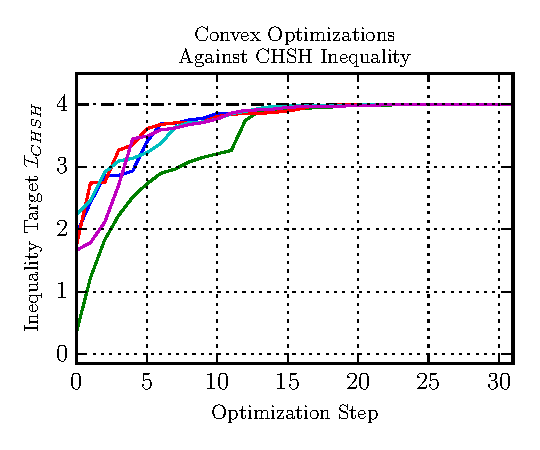
\includegraphics{../figures/CHSH_convex.pdf}
            \caption{Convex optimizations against $\mathcal{I}\tsb{CHSH}$ recover algebraic violation of $4$.}
            \label{fig:CHSH_convex}
        \end{minipage}\hspace{0.04\textwidth}%
        \begin{minipage}[b]{.48\textwidth}
            \centering
            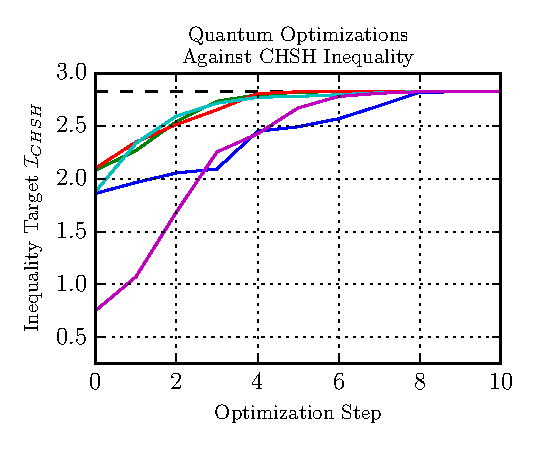
\includegraphics{../figures/CHSH_quantum.pdf}
            \caption{Quantum optimizations against $\mathcal{I}\tsb{CHSH}$ recover maximum violation of $2\sqrt{2}$.}
            \label{fig:CHSH_quantum}
        \end{minipage}
    \end{center}
    \end{figure}

    \todo[TC]{Demonstrate Quantum, Convexity}
    \todo[TC]{Why Inequalities are great for optimizations}
    \todo[TC]{Non-linearity}
    \todo[TC]{Techniques Used}
    \todo[TC]{Finding maximum violation of CHSH easily}
    \todo[TC]{Unreliance when number of parameters increases}
    \todo[TC]{Issues with local minimum}
    \todo[TC]{Using initial conditions close to fritz, obtain greater violation}
    \todo[TC]{Greater violation shares possibilistic structure of fritz and violates CHSH under definition}
    \todo[TC]{Not realizable with maximally entangled qubit states}
    \todo[TC]{Not realizable with separable measurements}
    \todo[TC]{Many non-trivial inequalities to be tested}
    \todo[TC]{inequality -> dist -> inequality evolution}
    \section{Conclusions}
    \todo[TC]{Inflation technique allows one to witness fritz incompatibility}
    \todo[TC]{Linear optimization induces certificates which are incompatibility witnesses}
    \todo[TC]{There are quantum distributions in the Triangle Scenario that are incompatible and different from fritz in terms of entanglement but not possibilistic structure}
    \section{Open Questions \& Future Work}
    \todo[TC]{Lots of stuff}
    \appendix
    \section{Exemplary Inequalities}
    \section{Connections to Sheaf-Theoretic Treatment}
    \section{Higher Order Logical Implications as a Complete Solution to the Marginal Problem}
    \section{Computationally Efficient Parametrization of the Unitary Group}
    Spengler, Huber and Hiesmayr \cite{Spengler_2010_Unitary} suggest the parameterization of the unitary group $\mathcal{U}\br{d}$ using a $d\times d$-matrix of real-valued parameters $\lambda_{n, m}$,
    \[ U = \bs{\prod_{m=1}^{d-1} \br{\prod_{n=m+1}^{d} \exp\br{i P_n \lambda_{n,m}}\exp\br{i \si_{m,n} \lambda_{m,n}}}} \cdot \bs{\prod_{l=1}^{d} \exp\br{iP_l \lambda_{l,l}}}  \eq \label{eq:spengler_unitary} \]
    Where $P_l$ are one-dimensional projective operators,
    \[ P_l = \ket{l}\bra{l} \eq \label{eq:projective_operator} \]
    and the $\si_{m,n}$ are generalized anti-symmetric $\si$-matrices,
    \[ \sigma_{m,n} = -i \ket{m}\bra{n} +i \ket{n}\bra{m} \]
    Where $1 \leq m < n \leq d$. Spengler et. al. proved the validity of \cref{eq:spengler_unitary} in Ref. \cite{Spengler_2010_Unitary}.

    For the sake of reference, let us label the matrix exponential terms in \cref{eq:spengler_unitary} in a manner that corresponds to their affect on an orthonormal basis $\bc{\ket{1}, \ldots, \ket{d}}$.
    \begin{align}
    \begin{split}
        GP_l &= \exp\br{iP_l \lambda_{l,l}} \\
        RP_{n,m} &= \exp\br{i P_n \lambda_{n,m}} \\
        R_{m,n} &= \exp\br{i \si_{m,n} \lambda_{m,n}}
    \end{split} \eq \label{eq:exp_terms}
    \end{align}
    It is possible to remove the reliance on matrix exponential operations in \cref{eq:spengler_unitary} by utilizing the explicit form of the exponential terms in \cref{eq:exp_terms}. As a first step, recognize the defining property of the projective operators \cref{eq:projective_operator},
    \[ P_l^k = \br{\ket{l}\bra{l}}^k = \ket{l}\bra{l} = P_l \]
    This greatly simplifies the global phase terms $GP_l$,
    \[ GP_l = \exp\br{iP_l \lambda_{l,l}} = \sum_{k=0}^{\inf} \f{\br{iP_l \lambda_{l,l}}^k}{k!} = \mathbb{I} + \sum_{k=1}^{\inf} \f{\br{i \lambda_{l,l}}^k}{k!}P_l^k = \mathbb{I} + P_l \bs{\sum_{k=1}^{\inf} \f{\br{i \lambda_{l,l}}^k}{k!}} = \mathbb{I} + P_l \br{e^{i \lambda_{l,l}} - 1} \eq \label{eq:unitary_GP} \]
    Analogously for the relative phase terms $RP_{n,m}$,
    \[ RP_{n,m} = \cdots = \mathbb{I} + P_n \br{e^{i \lambda_{n,m}} - 1} \eq \label{eq:unitary_RP} \]
    Finally, the rotation terms $R_{m,n}$ can also be simplified by examining powers of $i \sigma_{n,m}$,
    \[ R_{m,n} = \exp\br{i \si_{m,n} \lambda_{m,n}} = \sum_{k=0}^{\inf} \f{\br{\ket{m}\bra{n} - \ket{n}\bra{m}}^k \lambda_{m,n}^k}{k!} \]
    One can verify that the following properties hold,
    \begin{align*}
        \br{\ket{m}\bra{n} - \ket{n}\bra{m}}^0 &= \mathbb{I} \\
        \forall k \in \N, k \neq 0 : \br{\ket{m}\bra{n} - \ket{n}\bra{m}}^{2k} &= \br{-1}^k\br{\ket{m}\bra{m} + \ket{n}\bra{n}} \\
        \forall k \in \N : \br{\ket{m}\bra{n} - \ket{n}\bra{m}}^{2k+1} &= \br{-1}^k\br{\ket{m}\bra{n} - \ket{n}\bra{m}}
    \end{align*}
    Revealing the simplified form of $R_{m,n}$,
    \[ R_{m,n} = \mathbb{I} + \br{\ket{m}\bra{m} + \ket{n}\bra{n}} \sum_{j=1}^{\inf} \br{-1}^j\f{\lambda_{n,m}^{2j}}{\br{2j}!} + \br{\ket{m}\bra{n} - \ket{n}\bra{m}} \sum_{j=0}^{\inf} \br{-1}^j\f{\lambda_{n,m}^{2j+1}}{\br{2j+1}!} \]
    \[ R_{m,n} = \mathbb{I} + \br{\ket{m}\bra{m} + \ket{n}\bra{n}} \br{\cos\lambda_{n,m} - 1} + \br{\ket{m}\bra{n} - \ket{n}\bra{m}} \sin\lambda_{n,m} \eq \label{eq:unitary_R} \]
    By combining the optimizations of \cref{eq:unitary_RP,eq:unitary_R,eq:unitary_GP} together we arrive at an equivalent form for \cref{eq:spengler_unitary} that is computational more efficient.
    \[ U = \bs{\prod_{m=1}^{d-1} \br{\prod_{n=m+1}^{d} RP_{n,m}R_{m,n}}} \cdot \bs{\prod_{l=1}^{d} GP_l} \eq \label{eq:fast_spengler_unitary} \]
    In quantum mechanics, the global phase of a state $\ket{\psi} \in \Hilb^n$ is a \textit{redundant} parameter. Parameterizing unitaries using \cref{eq:fast_spengler_unitary} is especially attractive since the global phase terms $GP_l$ can be dropped, allowing one to parameterize all unitaries in $\mathcal{U}\br{d}$ up to this degeneracy \cite{Spengler_2010_Unitary}\footnote{In our implementation, we accomplish this by explicitly setting $\lambda_{l,l} = 0$ in \cref{eq:unitary_GP}}.
    \[ U_{/ GP_l} = \bs{\prod_{m=1}^{d-1} \br{\prod_{n=m+1}^{d} RP_{n,m}R_{m,n}}} \eq \label{eq:fast_spengler_unitary_gp} \]
    \todo[TC]{Explanation of Computational Complexity $\mathcal{O}\br{d^3}$ vs. $\mathcal{O}\br{1}$ using \cite{Moler_2003}}
    \todo[TC]{Pre-Caching for Fixed dimension $d$}
    \todo[TC]{Talk about inverse via haar measure}

    \section{Parametrization of Quantum States \& Measurements}
    Throughout \cref{sec:optimizations}, we utilize a variety of parameterizations of quantum states and measurements in order to generate quantum-accessible probability distributions. There are numerous techniques that can used when parameterizing quantum states and measurements \cite{Petz_2015, Hedemann_2013,Spengler_2010_Unitary,Fujii_2005,James_2001} with applications \todo[TC]{Finish this sentence}. For our purposes, we need to parameterize the space of quantum-accessible distributions $\prob[\mathcal{Q}]$ that are \textit{realized} on the Triangle Scenario. We have implemented $\prob[\mathcal{Q}]$ under the following description.
    \[ \prob[ABC]\br{abc} = \Tr\bs{\Omega^\intercal \rho_{AB}\otimes\rho_{BC}\otimes\rho_{CA} \Omega M_{A,a}\otimes M_{B,b} \otimes M_{C,c}} \eq \label{eq:triangle_quantum_distributions} \]

    \subsection{Quantum States}
    The bipartite states $\br{\rho_{AB}, \rho_{BC}, \rho_{CA}}$ of \cref{eq:triangle_quantum_distributions} were taken to be two-qubit density matrices acting on $\Hilb^2 \otimes \Hilb^2$.\footnote{We also considered qutrit $\Hilb^3$ qutit $\Hilb^4$ states. However for $6$ $d$-dimensional $\Hilb^d$ states, the joint density matrix $\rho$ acts on $\br{\Hilb^d}^{\otimes 6}$ making it a $\br{d^6, d^6}$ matrix with $d^{12}$ entries. Computationally only $d = 2$ was feasible for our optimization tasks.} The space of all such states corresponds to the space of all $4\times 4$ positive semi-definite hermitian matrices with unitary trace. Throughout this section, we refer to these bipartite states simply as $\rho$ unless otherwise indicated. There are three distinct techniques that we have considered.

    Taking inspiration from \cite{James_2001}, we can parameterize all such density matrices $\rho$ using \term{Cholesky Parametrization} \cite{Grasmair_2014}. The Cholesky decomposition allows one to write any hermitian positive semi-definite matrix $\rho$ in terms of a lower (or upper) triangular matrix $T$ using $\rho = T^\dagger T$. Our Cholesky parameterization consists of assigning $16$ real-valued parameters $\lambda$ to the entires of $T$ and generating a unitary trace $\rho$ similar to eq. (4.4) of \cite{James_2001}.
    \[ \rho = \f{T^\dagger T}{\Tr\br{T^\dagger T}} \quad T = \pmtrx{\la_{1}&0&0&0\\\la_{2} + i \la_{3}&\la_{4}&0&0\\\la_{5} + i \la_{6}&\la_{7} + i \la_{8}&\la_{9}&0\\\la_{10} + i \la_{11}&\la_{12} + i \la_{13}&\la_{14} + i \la_{15}&\la_{16}} \eq \label{eq:cholesky_param} \]
    Our deviation from exclusiving using \cref{eq:cholesky_param} is two-fold. First, \cref{eq:cholesky_param} is degenerate in that the normalization indicates only $16 - 1 = 15$ parameters are required for fully generic parameterization of all such states $\rho$. Removing this degeneracy is possible although difficult. Second, the parameters $\lambda_i$ carry no physical meaning associated with the state $\rho$, unlike our next parameterization.

    In Spengler, Huber and Hiesmayr's work \cite{Spengler_2010_Unitary}, they discuss how to parameterization density matrices $\rho$ acting on $\Hilb^d$ of rank $k$ through it's spectral decomposition,
    \[ \rho = \sum_{i=1}^{k} p_i \ket{\psi_i}\bra{\psi_i} \quad p_i \geq 0, \sum_{i} p_i = 1, k \leq d \eq \label{eq:unitary_param_density} \]
    Where any orthonormal basis $\bc{\ket{\psi_i}}$ of $\Hilb^d$ can be transformed into a computational basis $\bc{\ket{i}}$ by a unitary $U \in \mathcal{U}\br{d}$ such that $\ket{\psi_i} = U\ket{i}$. We refer to \cref{eq:unitary_param_density} as the \term{Spengler Parametrization}. Without loss of generality we parameterize all full-rank ($k=d$) matrices by simultaneously parameterizing the $d=4$ eigenvalues $p_i$ of \cref{eq:unitary_param_density} using \cref{eq:convex_param} and the unitary group $\mathcal{U}\br{4}$ up to global phase equivalence using \cref{eq:fast_spengler_unitary_gp}. Parameterizing $\rho$ using the Spengler parameterization requires $3 + 12 = 15$ parameters; admitting no degeneracies.

    Finally in cases where we wish to restrict ourselves to \textit{pure} bipartite states $\rho = \ket{\psi}\bra{\psi}$, we have the luxury to use a \term{Schmidt Parametrization}. This is accomplished via a Schmidt decomposition $\ket{\psi_{AB}} = \sum_{i}\sigma_i \ket{i_A}\otimes\ket{i_B}$ where normalization demands that $\sum_{i} \sigma_i^2 = 1$, $\bc{\ket{i_A}}$ and $\bc{\ket{i_B}}$ are orthonormal bases for $\Hilb_A$ and $\Hilb_B$ respectively \cite{Neilsen_Chaung_2011}. Additionally for qubit sources we can \textit{choose} our orthonormal bases to be the computational basis $\bc{\ket{0}, \ket{1}}$ and write,
    \[ \ket{\psi} = \cos^2\br{\lambda_1} \ket{0} \otimes \ket{0} + \sin^2\br{\lambda_1} \ket{1} \otimes \ket{1} \]
    Where only $1$ real-valued parameter $\lambda = \bc{\lambda_1}$ is required to parameterize all pure states up to local unitaries. Pure states are also attractive due to their computational advantage in computing \cref{eq:triangle_quantum_distributions}. If each state $\rho$ is decomposable into $\ket{\psi}\bra{\psi}$, then \cref{eq:triangle_quantum_distributions} can be written as,
    \[ \prob[ABC]\br{abc} = \bramidket{\psi_{AB}\psi_{BC}\psi_{CA}}{\Omega M_{A,a}\otimes M_{B,b} \otimes M_{C,c} \Omega^\intercal}{\psi_{AB}\psi_{BC}\psi_{CA}} \eq \label{eq:pure_state_quantum_triangle} \]
    Avoiding the expensive matrix multiplications of \cref{eq:triangle_quantum_distributions}.
    \subsection{Measurements}
    With full generality, we consider a measurement $M$ to be a \term{projective-operator valued measure (POVM)} represented by a set of hermitian, positive semi-definite operators $\bc{M_i}_{i=1,\ldots,k}$\footnote{The $i$-th element of $M$ is referenced using a subscript $M_i$. The set of measurement elements for a particular party $X$ will be written $M_X$. When both party and element are to be referenced, we write $M_{X,i}$.} acting on $\Hilb^d$ summing to the identity,
    \[ \forall \ket{\phi} \in \Hilb^d : \bra{\phi} M_i \ket{\phi} \geq 0 \quad \sum_{i=1}^{k} M_i = \mathbb{I}_{\Hilb^d} \eq \label{eq:povm} \]
    When considering $k=2$ outcome measurements acting on $\Hilb^4$ we parameterize the first POVM element $M_1$ by using a Cholesky parameterization similar to \cref{eq:cholesky_param} without normalizing for trace. Afterwards, $M_2$ is fully determined by \cref{eq:povm}.
    \[ M_1 = T^\dagger T \quad M_2 = \mathbb{I} - T^\dagger T \eq \label{eq:2_povm}\]
    However, in order for $M_2$ to be positive semi-definite, the largest eigenvalue of $M_1$ has to be less than 1. To see this is a necessary and sufficient constraint, first expand out \cref{eq:2_povm},
    \[ \bramidket{\phi}{M_2}{\phi} = \bramidket{\phi}{\mathbb{I} - M_1}{\phi} = \abs{\phi}^2 - \bra{\phi}\br{\sum_{i=1}^{d}m^{\br{i}}_1 \ket{m^{\br{i}}_1}\bra{m^{\br{i}}_1}}\ket{\phi} \]
    Next write a generic $\ket{\phi} \in \Hilb^d$ in terms of a linear combination of the eigenvectors of $M_1$\footnote{The eigenvectors of $M_1$ form an orthonormal basis for $\Hilb^d$ because $M_1$ is Hermitian}.
    \[ \bramidket{\phi}{M_2}{\phi} = \sum_{j}\abs{\braket{\phi}{m^{\br{j}}_1}}^2 - \sum_{i} m^{\br{i}}_1 \abs{\braket{\phi}{m^{\br{i}}_1}}^2 = \sum_{i} \br{1 - m^{\br{i}}_1} \abs{\braket{\phi}{m^{\br{i}}_1}}^2 \eq \label{eq:eigen_less_one} \]
    Since $\ket{\phi}$ is arbitrary, for each $i$ set $\ket{\phi} = \ket{m^{\br{i}}_1}$ to see that each eigenvalue of $M_1$ needs to be less than $1$.
    \[ \bramidket{m^{\br{i}}_1}{M_2}{m^{\br{i}}_1} = \br{1 - m^{\br{i}}_1} \geq 0 \implies m^{\br{i}}_1 \leq 1 \eq \label{eq:2_povm_suff} \]
    By \cref{eq:eigen_less_one} is not difficult to see that \cref{eq:2_povm_suff} is a sufficient condition. During optimization, \cref{eq:2_povm_suff} can either be enforced passively as a constraint or directly by normalizing $M_1$ by its largest eigenvalue $\max\br{m_1^{\br{i}}}$ whenever necessary.

    When generalizing the above parameterization to more than $2$ outcomes, only necessary conditions were found. Generating $k$-outcome POVM measurements is doable using rejection sampling techniques such as those used in \cite{Petz_2012} however a valid parameterization with little to no degeneracy was not found. Upon making this observation, a necessary departure to \term{projective-valued measures (PVMs)} is warranted\footnote{Strictly speaking, when the number of outcomes ($k$) \textit{matches} the Hilbert space dimension ($d$), \cref{eq:povm} implies \cref{eq:pvm} by completeness. When considering $4$ outcome measurements on bipartite qubit states in $\Hilb^4$, PVMs are completely general. Moreover, Naimark's dilation theorem guarantees that PVMs acting on $\Hilb^q$ can \textit{emulate} the behaviour of any POVM acting on $\Hilb^d$ provided that $q$ is sufficiently larger than $d$ \cite{Naimark}.}. With loss of generality, consider the set of PVMs $M$ satisfying \cref{eq:povm} in addition to orthogonal and projective properties,
    \[ M_i M_j = \de_{ij} M_i \quad M_i = \ket{m_i}\bra{m_i} \eq \label{eq:pvm}\]
    Parameterizing $M$ for $k$-outcome measurements corresponds to parameterizing the set of all $k$-th order orthonormal sub-bases of $\Hilb^d$.
    First note that any such basis $\bc{\ket{\psi_1}, \ldots, \ket{\psi_k}}$ can be transformed into the computational basis $\bc{\ket{1}, \ldots, \ket{k}}$ by a unitary denoted $U \in \mathcal{U}\br{d}$,
    \[ U \ket{\psi_i} = \ket{i} \]
    With this observation we just need to parameterize the set of all unitaries $\mathcal{U}\br{d}$,
    \[ M = \bc{ U\ket{i}\bra{i}U^\dagger }_{i \in 1, \ldots, k} \]
    Specifically, the projective property each $M_i$ means that the global phase of $U$ is completely arbitrary; one only needs to consider parameterizing unitaries up to global phase \cref{eq:fast_spengler_unitary_gp}. This method was inspired by the \textit{measurement seeding} method of P{\'{a}}l and V{\'{e}}rtesi's \cite{Pal_2010} iterative optimization technique.

    Analogously to \cref{eq:pure_state_quantum_triangle}, projective measurements offer considerable computational advantage as \cref{eq:triangle_quantum_distributions} can be rewritten as,
    \[ \prob[ABC]\br{abc} = \bramidket{m_{A,a}m_{B,b}m_{C,c}}{\Omega^\intercal \rho_{AB}\otimes\rho_{BC}\otimes\rho_{CA} \Omega}{m_{A,a}m_{B,b}m_{C,c}} \eq \label{eq:pure_meas_quantum_triangle} \]

    \subsection{Network Permutation Matrix}
    \begin{figure}
        \centering
        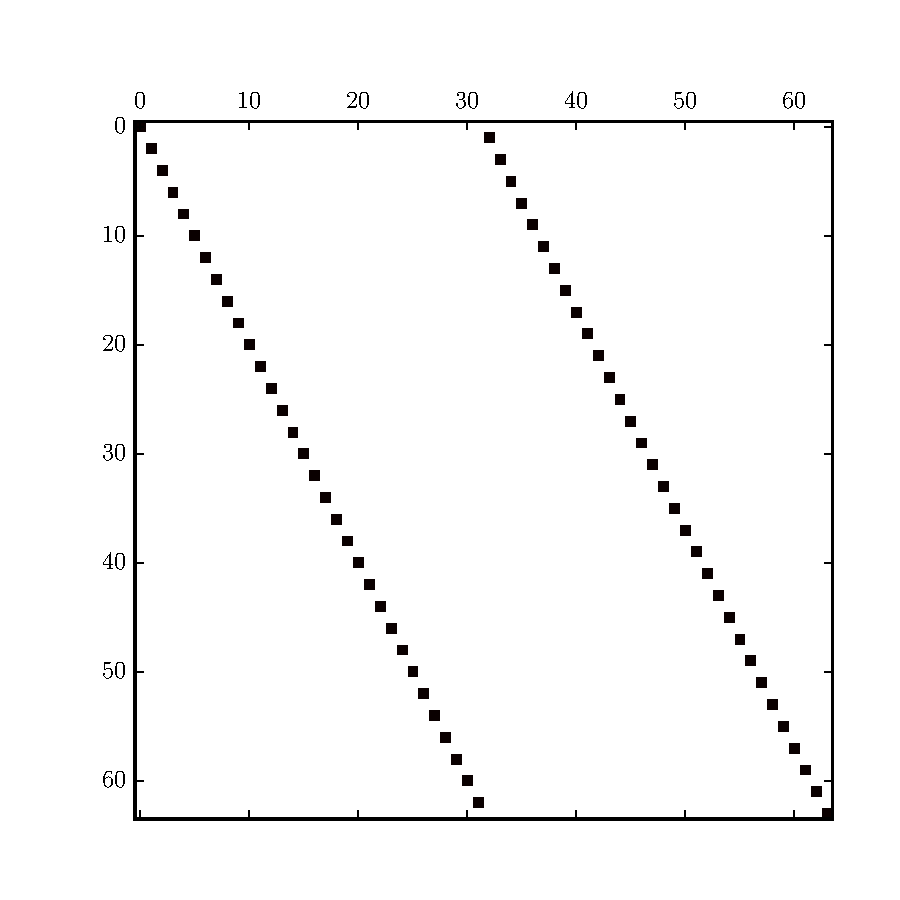
\includegraphics[trim={1cm 1.2cm 1.0cm 1cm},clip,width=0.4\textwidth]{../figures/perm_mtrx.pdf}
        \caption{The network permutation matrix $\Omega$ for $\br{\Hilb^2}^{\otimes 6}$ realized on the triangle scenario. Black represents a value of $1$ and $0$ otherwise.}
        \label{fig:perm_mtrx}
    \end{figure}
    Finally, we introduce the \term{network permutation matrix} $\Omega$ for the Triangle Scenario of \cref{fig:triangle_scenario}. For bipartite qubit states, $\Omega$ becomes a $64\times64$ bit-wise matrix that acts on the measurements $M$ and is depicted in \cref{fig:perm_mtrx}. To illuminate its necessity, consider \cref{eq:triangle_quantum_distributions} without $\Omega$.
    \begin{align*}
    \prob[ABC]\br{abc} &\stackrel{?}{=} \Tr\bs{\br{\rho_{AB}\otimes\rho_{BC}\otimes\rho_{CA}} \br{M^a_{A}\otimes M^b_{B} \otimes M^c_{C}}}\\
    &= \Tr\bs{\br{\rho_{AB}M^a_{A}}\otimes\br{\rho_{BC}M^b_{B}}\otimes\br{\rho_{CA}M^c_{C}}}\\
    &= \Tr\br{\rho_{AB}M^a_{A}}\Tr{\br{\rho_{BC}M^b_{B}}}\Tr{\br{\rho_{CA}M^c_{C}}}\\
    &= \prob[A\mid \rho_{AB}]\br{a}\prob[B\mid \rho_{BC}]\br{b}\prob[C\mid \rho_{CA}]\br{c}
    \end{align*}
    On an operational level, this corresponds to $A$ making a measurement on \textit{both} subsystems of $\rho_{AB}$ and \textit{not} on any component of $\rho_{CA}$. This is analogously troubling for $B$ and $C$ as well. The network permutation matrix $\Omega$ corresponds to \textit{aligning} the underlying $6$-qubit joint state $\rho$ with the joint measurement $M$. To understand its effect, consider its effect on $6$-qubit pure state $\ket{q_1} \otimes \cdots \otimes \ket{q_6} = \ket{q_1q_2q_3q_4q_5q_6}$ where $\forall i : \ket{q_i} \in \Hilb^2$.
    \[ \Omega\ket{q_1q_2q_3q_4q_5q_6} = \ket{q_2q_3q_4q_5q_6q_1} \]
    $\Omega$ acts as a \textit{partial transpose} on $\br{\Hilb^2}^{\otimes 6}$ by shifting the underlying tensor structure one subsystem to the ``left''. It is uniquely defined by its action on all $2^6$ orthonormal basis elements of $\br{\Hilb^2}^{\otimes 6}$,
    \[ \Omega \defined \sum_{\ket{q_i} \in \bc{\ket{0}, \ket{1}}}\ket{q_2q_3q_4q_5q_6q_1}\bra{q_1q_2q_3q_4q_5q_6} \]
    \subsection{Degeneracy}
    \todo[TC]{Discuss local unitary degeneracy}
    \section{Convex Parametrization of Finite Probability Distributions}
    As discussed in \cref{sec:optimizations}, there is a need to parameterize the family of all probability distributions $\prob[V]$ over a given set of variables $V = \br{v_1, \ldots, v_{\abs{V}}}$. If the cardinality of $O_{V}$ is finite, then this computationally feasible. The space of probability distributions over $n = \abs{O_{V}}$ distinct outcomes forms a $n-1$ dimensional convex polytope naturally embedded in $\R_{\geq 0}^n$ \cite{Brunner_2013} that is parameterizable by $n-1$ real value parameters; normalization $\sum_{o\bs{V} \in O_V} \prob[V][\outc{V}] = 1$ accounts for the `$-1$'. An example of a non-degenerate parameterization of $\prob[V]$ consists of $n-1$ parameters $\lambda = \br{\lambda_1, \ldots, \lambda_{n-1}}, \lambda_i \in \bs{0, \pi/2}$ which generate the $n$ probability values $p_j$ using hyperspherical coordinates \cite{Hedemann_2013, Spengler_2010_Unitary},
    \begin{equation}
    \begin{gathered}
        \label{eq:convex_param}
        p_j = \cos^2 \lambda_j \prod_{i=1}^{j-1} \sin^2 \lambda_i \quad \forall j \in 1, \ldots, n - 1 \\
        p_n = \prod_{i=1}^{n-1} \sin^2 \lambda_i
    \end{gathered}
    \end{equation}
    Furthermore due to the periodicity of the parameter space $\lambda$, \cref{eq:convex_param} can be used for either constrained or unconstrained optimization problems. For continuity reasons, unconstrained optimizations are performed whenever possible.

    Although non-degenerate, this parameterization suffers from uniformity; a randomly sampled vector of parameters $\lambda$ \textit{does not} translate to a randomly sampled probability $\prob[V]$. An easy-to-implement, degenerate parameterization of $\prob[V]$ can be constructed by simply beginning with $n$ real parameters $\lambda = \br{\lambda_1, \ldots, \lambda_n}$, then making them positive and normalized by their sum\footnote{Strictly speaking, \cref{eq:uniform_param} \textit{also} suffers from non-uniformity; being biased toward uniform probability distributions $\prob[V]$. \todo[TC]{Discuss rejection sampling simplex algorithms}}.
    \[ p_j = \f{\abs{\lambda_j}}{\sum_{i=1}^{n} \abs{\lambda_i}} \quad \forall j \in 1, \ldots, n \eq \label{eq:uniform_param} \]
    For various convex optimization tasks sensitive to initial conditions outlined \cref{sec:optimizations}, the latter parameterization of \cref{eq:uniform_param} generally performed better than the former \cref{eq:convex_param}.

    \bibliography{references}
\end{document}